% =====================================================================
%  var-task-rep -- Minimal proposal skeleton
%  One grey box per section. Add \subsection{...} freely inside any
%  section; each new subsection can carry its own box: \ph{ID}{title}{notes}.
% =====================================================================
\documentclass[11pt,a4paper]{article}

\usepackage[utf8]{inputenc}
\usepackage[T1]{fontenc}
\usepackage[margin=2.5cm]{geometry}
\usepackage{amsmath,amssymb,amsthm}
\usepackage{booktabs}
\usepackage{graphicx}
\usepackage{fvextra}
\DefineVerbatimEnvironment{promptbox}{Verbatim}{breaklines,breakanywhere,fontsize=\footnotesize,frame=single,framesep=2mm}
\usepackage{xcolor}
\usepackage[most]{tcolorbox}
\usepackage[round,authoryear]{natbib}
\usepackage[colorlinks=true,linkcolor=blue!50!black,citecolor=green!40!black,urlcolor=blue!60!black]{hyperref}

% Placeholder box: \ph{ID}{What goes here}{Notes}
\definecolor{phframe}{gray}{0.55}
\definecolor{phback}{gray}{0.95}
\newcommand{\ph}[3]{%
  \hypertarget{ph:#1}{}%
  \begin{tcolorbox}[enhanced,breakable,colback=phback,colframe=phframe,
    boxrule=0.4pt,arc=1mm,left=2mm,right=2mm,top=1mm,bottom=1mm,
    fonttitle=\sffamily\small\bfseries,coltitle=black,colbacktitle=gray!25,
    title={[#1]\quad TO WRITE --- #2}]
  \small #3
  \end{tcolorbox}}

% Inline value to be decided
\newcommand{\tbd}[1]{\textcolor{red!70!black}{\textsf{[TBD: #1]}}}

% Link back to the status table, placed under each section heading
\newcommand{\backtostatus}{\noindent{\hfill\footnotesize\hyperref[sec:status]{$\uparrow$\,status}}\par}

% Status row: \strow{label}{name}{content}{status}
\newcommand{\strow}[4]{\hyperref[#1]{#2} & #3 & #4 \\}

\newtheorem{definition}{Definition}
\newtheorem{hypothesis}{Hypothesis}

\title{Lexical Task Heads beyond Simple Tasks:\\ Logit Lens and Jacobian Lens Readouts}
\author{Filippo Merlo}
\date{Draft --- \today}

\begin{document}
\maketitle

\begin{abstract}
\phantomsection\label{sec:abstract}
Lexical task heads are attention heads whose output, decoded into the vocabulary, names the task the prompt asks for \citep{yang2026shared}. They were identified with the per-head logit lens on simple single-step tasks, such as mapping a country to its capital. We ask whether the same method finds them for complex tasks defined by explicit rules \citep{fu2026rules}, which need several inference steps, and whether Head-JLens \citep{merlo2026headjlens}, which decodes each head's output after mapping it through a Jacobian of the remaining layers averaged over many texts, finds lexical task heads that the logit lens misses. In Llama-3.1-8B-Instruct, we identify lexical task heads under both readouts on 14 simple tasks and 5 complex tasks at their easy level, with rule-based and example-based prompts, and test each head set by activation patching.
\end{abstract}

\section{Introduction}\label{sec:intro}
A language model's accuracy on a task can change a great deal with the wording of the prompt that asks for it: on Llama-3.1-8B-Instruct, prompts for the same antonym items differ in accuracy by up to a factor of four \citep[Fig.~1]{yang2026shared}. \citet{yang2026shared} explain part of this variation with \emph{lexical task heads}, attention heads whose outputs, decoded into the vocabulary with the logit lens, name the task (``opposite'' for antonyms, ``cities'' for capitals). The heads are largely shared between instruction-based and example-based prompts, patching their mean activation into a prompt without task information raises task accuracy, and prompts that fail activate them less.

Two limits of that work motivate this project. First, its 17 tasks are simple single-step mappings (country to capital, word to antonym), and the authors note that ``it remains unclear if these shared lexical mechanisms hold for more abstract tasks or tasks that are less easily defined by simple vocabulary clusters'' \citep[Sec.~4]{yang2026shared}. \citet{fu2026rules} provide such tasks: five novel tasks defined by explicit rules (a card game, a board game, a composed arithmetic operator, noun-class agreement in an artificial language, and lexical-category inference), each at three difficulty levels and each given as rules, as examples or as both. Second, the logit lens decodes a head's output directly and leaves out the computation of the layers that follow it; \citet[Sec.~4]{yang2026shared} note that task representations ``encoded in a non-lexical, abstract format'' may not project cleanly to tokens. Head-JLens reads each head through a Jacobian map of the remaining layers, and on Llama-3.1-8B-Instruct it ranks annotated intermediate words, which the prompt never states (such as the bridge entity of a two-hop question), higher than the per-head logit lens at most layers on five of six evaluation sets \citep[Sec.~3]{merlo2026headjlens}.

We therefore ask whether \citeauthor{yang2026shared}'s method identifies lexical task heads for the complex tasks of \citet{fu2026rules}, and how the logit lens and Head-JLens compare as readouts for identifying them.

\paragraph{Contributions.}
\begin{enumerate}
\item A test of the lexical-task-head method on complex, rule-defined tasks, with a causal check of the identified heads.
\item A comparison of the per-head logit lens and Head-JLens for identifying lexical task heads, on simple and complex tasks.
\end{enumerate}

\section{Related work}\label{sec:background}
\paragraph{Task representations across prompting styles.} Function vectors are sums of the mean outputs of a few attention heads that, added to the residual stream, trigger a task in another context \citep{todd2024function}. \citet{davidson2025different} extract them from instructions as well as from demonstrations and find that the two prompting styles engage mostly different heads: of the 20 top heads in each model, 2 to 7 are shared. \citet{yang2026shared} identify a different kind of task representation, lexical task heads, whose outputs decode to words describing the task; 73\% of them are shared between instruction-based and example-based prompts on average, and they are largely disjoint from function-vector heads \citep[App.~I]{yang2026shared}. We test the lexical-task-head method on complex tasks.

\paragraph{Reading attention heads in the vocabulary.} The logit lens decodes an intermediate state with the model's final normalization and unembedding \citep{nostalgebraist2020logitlens}; applied to one head's output, it is the readout of \citet{yang2026shared}. The Jacobian lens of \citet{gurnee2026workspace} instead maps a residual-stream state through a Jacobian of the remaining layers, averaged over many texts. Head-JLens moves this map to the concatenated head outputs, so that each head is read through the layers that follow it; in Llama-3.1-8B-Instruct it ranks annotated intermediate words higher than the per-head logit lens at most layers on five of six evaluation sets, and heads selected with it are better sites for edits \citep{merlo2026headjlens}. We compare the two readouts on a different use: identifying task-descriptive heads.

\paragraph{Learning tasks from rules and from examples.} \citet{fu2026rules} compare learning from rules, from examples and from both on five novel tasks. Rules outperform examples overall, adding examples to rules gives no significant gain, and the advantage of rules is largest for tasks that need algebraic computation. Their study is behavioural; we use their tasks to study task representations.

\section{Research questions}\label{sec:rq}
\begin{description}
\item[RQ1] Does the method of \citet{yang2026shared} identify lexical task heads for the complex tasks of \citet{fu2026rules} under rule-based and example-based prompts, and do the identified heads have a causal effect on task accuracy?
\item[RQ2] How do the per-head logit lens and Head-JLens compare as readouts for identifying lexical task heads, on simple and on complex tasks?
\item[RQ3] Are the lexical task heads of a complex task shared between rule-based and example-based prompts, as \citet{yang2026shared} find for simple tasks?
\end{description}

\begin{hypothesis}[replication]\label{h:rep}
On the simple tasks, Logit-head reproduces \citet{yang2026shared}: lexical task heads are found for every task, and patching them into prompts without task information raises accuracy above the unpatched baseline. \emph{Falsified} if, on the same model, the method finds no heads or no accuracy gain for tasks where \citet{yang2026shared} report both.
\end{hypothesis}

\begin{hypothesis}[complex tasks]\label{h:complex}
Following the limitation stated by \citet[Sec.~4]{yang2026shared}, the complex tasks yield fewer lexical task heads per task and a smaller causal effect than the simple tasks under Logit-head. \emph{Falsified} if they yield as many heads with as large an effect.
\end{hypothesis}

\begin{hypothesis}[readouts]\label{h:readout}
Following \citet{merlo2026headjlens}, J-head identifies at least the lexical task heads that Logit-head identifies, and the heads found only by J-head have a causal effect above baseline. \emph{Falsified} if the J-head set misses heads of the Logit-head set, or if the heads found only by J-head have no causal effect.
\end{hypothesis}

\paragraph{Scope.} We do not explain behavioural variation across wordings (the failure analyses of \citealp[Sec.~2.4]{yang2026shared}), and we use one model.

\section{Framework}\label{sec:framework}
\paragraph{Tasks and prompts.} A task $t$ is given by a dataset $D_t$ of inputs and correct outputs. For the complex tasks we use the easy level of each (Sec.~\ref{sec:tasks}). Each prompt for $t$ has a style $s\in\{\text{rule},\text{example},\text{combined}\}$: its task information is a rule text, a set of demonstrations, or both, followed by the input $x$. $P_{t,s}$ is the set of prompts of style $s$ for $t$, and $P^{+}_{t,s}\subseteq P_{t,s}$ the prompts whose heads are read: those the model answers correctly under the flexible score of Sec.~\ref{sec:evaluation}, for both families of tasks, whether or not the answer is the first generated text.

\paragraph{Heads and readouts.} Following \citet[Sec.~2]{merlo2026headjlens}, $z_{l,h}(p)$ is the output of head $h$ in layer $l$ at the last position of $p$, before the output projection, and $c_{l,h}(p)=W^{(h)}_{O,l}z_{l,h}(p)$ its write to the residual stream. With $q_v=g\odot w_v$ the gain-scaled unembedding row of token $v$, the two readouts score $v$ by
\[
\ell^{\mathrm{L}}_{l,h}(p)[v]=q_v^\top c_{l,h}(p)\quad\text{(Logit-head)},\qquad
\ell^{\mathrm{J}}_{l,h}(p)[v]=q_v^\top J_{l,h}\,z_{l,h}(p)\quad\text{(J-head)}.
\]
$T^{R}_{k,l,h}(p)$ is the set of the $k$ highest-scoring tokens under readout $R\in\{\mathrm{L},\mathrm{J}\}$, and $V_t$ the term list of task $t$.

\begin{definition}[Lexical task head]\label{def:lth}
Following \citet[Sec.~2.2.2]{yang2026shared}, head $(l,h)$ is a lexical task head for $t$ on prompt $p$ under readout $R$ if $|T^{R}_{k,l,h}(p)\cap V_t|\geq n$. It is a lexical task head for $t$ and style $s$ if this holds for at least a fraction $\rho$ of the prompts in $P^{+}_{t,s}$. We use $n=1$, $k=10$, $\rho=0.1$, as \citet{yang2026shared}. $H^{R}_{t,s}$ denotes the set of such heads.
\end{definition}

\section{Methods}\label{sec:methods}

\subsection{Model}\label{sec:model}
Llama-3.1-8B-Instruct: it is the main model of \citet{yang2026shared}, and the only model with released Head-JLens matrices.

\subsection{Tasks}\label{sec:tasks}
\paragraph{Simple tasks.} The 14 tasks used by both \citet{yang2026shared} and \citet{davidson2025different}, with the datasets of \citet{todd2024function}: antonym, synonym, singular--plural, present--past, country--capital, country--currency, landmark--country, park--country, product--company, next-item, prev-item, English--French, English--German, English--Spanish.
Rule-based prompts: the five instruction templates per task of \citet[App.~A.3.1]{yang2026shared}.
Example-based prompts: 1, 5, 10, 20 and 30 shots \citep[App.~A.3]{yang2026shared}.

\paragraph{Complex tasks.} The five tasks of \citet{fu2026rules} at their easy level: Set Game, Tapatan, Operator Function, Noun Class Agreement, Lexical Category Inference. Data from their public release: 300 test items per task, drawn with their sampler and seed (all 600 for Lexical Category Inference), the same items under every prompt.
Rule-based prompts: their rules-only prompts \citep[App.~F]{fu2026rules} and further wordings (Sec.~\ref{sec:trmethods}).
Example-based and combined prompts: their minimum-coverage demonstration sets \citep[Sec.~2.5]{fu2026rules}.

\paragraph{Why these tasks.} Lexical task heads and their term lists were defined on the simple tasks \citep{yang2026shared}, so the method applies unchanged and our results can be compared with theirs. \citet[Sec.~4]{yang2026shared} restrict their study to tasks with simple lexical descriptions. The complex tasks are novel, need several inference steps, and are given in rule, example and combined forms that specify the same task on the same test items, so the task is held fixed while the way it is communicated varies \citep[Sec.~1--2]{fu2026rules}.

\paragraph{Answer format.} As in the source studies: the templates of \citet{yang2026shared} for the simple tasks, and the answer formats of \citet[App.~F]{fu2026rules} for the complex tasks, under the chat template. Decoding is greedy, as in \citet[App.~A]{fu2026rules} (temperature 0; their released code defaults to 0.1), so that the prompt whose heads are read and the scored answer always match. The five complex tasks are generated alike (Sec.~\ref{sec:reasoning}): the model may explain or reason before it answers, as \citeauthor{fu2026rules}'s instruction-tuned models often do. Lexical task heads are read at the last prompt token, before any generated text, for every task.

\subsection{Task-representation methods}\label{sec:trmethods}
\paragraph{Lexical task heads} \citep[Sec.~2.2.2]{yang2026shared}.
Each attention head's output at the last prompt token is decoded with the two readouts of Sec.~\ref{sec:framework}: Logit-head, the per-head logit lens used by \citet{yang2026shared} \citep{nostalgebraist2020logitlens}, and J-head (Head-JLens), which applies the head's columns $J_{l,h}$ of the per-layer Jacobian map fitted on WikiText-103 \citep[Sec.~2]{merlo2026headjlens}. Fitted matrices for Llama-3.1-8B-Instruct are released with \citet[Sec.~S4]{merlo2026headjlens}.
Under each readout, lexical task heads are identified with Definition~\ref{def:lth}.
For the simple tasks, $P^{+}_{t,s}$ is taken as in the code of \citet{yang2026shared}: the first 100 prompts in $P^{+}$ under one wording, the 5-shot prompts for the example style and the instruction template with the highest accuracy for the rule style. The complex tasks follow the same rule: the first 100 such prompts under the most accurate rule wording, under the example-based prompts and under the combined prompts.
Term lists: \citet[App.~A.2.1]{yang2026shared} for the simple tasks; for the complex tasks, see below.

\paragraph{Simple tasks as in the source code.} The simple tasks are run as in the code of \citet{yang2026shared}, with three departures. First, padding: their code passes prompts to the model in batches of 20, padded on the left, without an attention mask, so that the model attends to the padding; we pass the mask and the matching positions, so that each prompt is computed as if run alone. Second, the J-head readout. Third, the precision of the forward pass: bfloat16, in which the Head-JLens matrices were fitted.

\paragraph{What we add to the complex tasks.}\label{sec:adapt} \citet{fu2026rules} provide the data, one rules-only prompt per task and difficulty level, and the example-based and combined prompts. To apply lexical task heads to them we add three things.
\begin{enumerate}
\item \emph{Rule wordings}: six per original rule prompt (App.~\ref{app:orig}), each stating exactly the same rules. They are generated with GPT-5.5 through the Azure OpenAI API from a paraphrase prompt that keeps placeholders, output labels and the answer-format instruction verbatim (App.~\ref{app:genprompts}), and each is checked by us against the original; App.~\ref{app:wordings} lists them. \citet{yang2026shared} use five instruction templates per simple task; the complex tasks have six rule wordings besides the original, and their rule-style $P^{+}$ is taken from the most accurate of the seven.
\item \emph{Term lists} of task-descriptive words, of the kind in \citet[App.~A.2.1]{yang2026shared}: single words that describe the task rather than its answers, with case and number variants. They are generated with GPT-5.5 through the Azure OpenAI API from the rule prompt (App.~\ref{app:genprompts}), as \citet[App.~O]{yang2026shared} generated term lists with LLMs, and checked by us. Each word is expanded to token ids as in \citet{yang2026shared}: as written, with a leading space, in upper, capitalised and lower case, and after a \texttt{.}, \texttt{\_} or \texttt{-}, keeping every variant that is a single token of the model's tokenizer. There is one list per original rule prompt (App.~\ref{app:orig}): Tapatan's levels share one prompt and change only board size, piece count and line length, whereas the other tasks add rules or, for Operator Function, change the function \citep[Table~1, App.~F]{fu2026rules}. Lists are task-specific, not item-specific: for Lexical Category Inference, whose category definitions change from item to item, the list contains only words that describe the task itself. App.~\ref{app:terms} lists them.
\item \emph{Prompts without task information} for the causal check (Sec.~\ref{sec:causal}): the input block of the rules-only prompt alone (the lines that introduce the input and the answer, such as \texttt{Sentence: \{sentence\}} and \texttt{Answer:}), without rules or examples, the counterpart of the zero-shot prompts of \citet[Sec.~2.3.2]{yang2026shared}.
\end{enumerate}

\paragraph{Generation and scoring of the complex tasks.}\label{sec:reasoning} All five complex tasks are run in one way: chat template, greedy decoding, and a reply that ends at the end-of-sequence token or at 1,024 new tokens. \citeauthor{fu2026rules} give instruction-tuned models longer limits (6,000 new tokens for Operator Function, App.~A). In an earlier run with that limit on Set Game, Operator Function and Tapatan (ten prompt variants, 300 items), 4 of 9,000 replies reached a correct answer after token 1,024, and 690 of the 804 longer replies ran to 6,000 tokens without one. The strict score is the evaluation of \citet{fu2026rules} on the whole reply: for Set Game and Operator Function, after whitespace is collapsed, the first \texttt{\textbackslash boxed\{\}}, read as three cards of the form \texttt{(animal | biome | \ldots)} or as an integer; for Noun Class Agreement, the first line that is only Yes or No (after an optional \texttt{Answer:}), else a line that begins \texttt{Answer:} or \texttt{Final answer:} followed by Yes or No, else the first Yes or No anywhere in the reply; for Lexical Category Inference, the reply's first word, which must be Yes or No. Their code has no scorer for Tapatan (it stores the reply only), and their paper describes none; its prompt asks for the label alone. We read the first of its three labels (\texttt{A win}, \texttt{B win}, \texttt{continue}) anywhere in the reply, as in our first run of E0. A reply without an extractable answer is wrong. Where items share a prompt (Tapatan's sample repeats 46 boards, Noun Class Agreement's 52 sentences), the prompt is answered once and its reply scored for each of them.

\paragraph{Why these readouts.} Lexical task heads locate a task representation and give its content in words \citep{yang2026shared}. Logit-head reproduces their readout. J-head reads each head through the layers that follow it: in Llama-3.1-8B-Instruct it ranks unstated intermediate words higher than Logit-head at most layers on five of six evaluation sets, and its readouts are better guides for edits \citep[Secs.~3--4]{merlo2026headjlens}. A lexical task head's decoded task word is likewise not the answer, and \citet[Sec.~4]{yang2026shared} note that their logit-lens criterion may miss task representations that do not project cleanly to tokens.

\subsection{Causal check}\label{sec:causal}
The causal check of \citet[Sec.~2.3.2, App.~G]{yang2026shared} tests whether a head set carries the task: the heads' mean output on task prompts is written into prompts that do not state the task, and we measure whether the model then performs it.
\begin{enumerate}
\item \emph{Patched prompts}: prompts without task information, the zero-shot prompts of \citet{yang2026shared} for the simple tasks and the input blocks of Sec.~\ref{sec:adapt} for the complex tasks, for items that the model answers correctly when the task is given. Their unpatched accuracy is the baseline.
\item \emph{Mean output}: for each head in the set, the mean of $c_{l,h}$ over the first 100 prompts of a wording answered correctly, leaving out the patched items. As in the code of \citet{yang2026shared}, each wording of a style (each instruction template, each number of shots, each rule wording) gives its own mean and its own patch.
\item \emph{Patch}: at the last position of each patched prompt, the output of every head in the set is replaced by its mean output times a scaling factor $\alpha$: for the simple tasks $\alpha\in\{-10,-6,-4,-2,0,1,2,\dots,10\}$, the values of \citet{yang2026shared}; for the complex tasks, whose replies run to 1,024 tokens, their even values and 1, $\alpha\in\{-10,-6,-4,-2,0,1,2,4,6,8,10\}$. The model answers from the patched prompt, generated as the saved outputs of Sec.~\ref{sec:evaluation}, and the answer is scored by the flexible score. For the simple tasks this replaces the first generated token, which the code of \citet{yang2026shared} reads; the first-token score is kept beside it.
\item \emph{Control}: the same patch at the same heads, with the mean output of a different task. A head set carries the task if its own mean raises accuracy and the control mean does not; a gain under both points to the answer format rather than the task.
\end{enumerate}
Three head sets are patched for each task and style: $H^{\mathrm{L}}_{t,s}$, $H^{\mathrm{J}}_{t,s}$, and the heads found only by J-head, $H^{\mathrm{J}}_{t,s}\setminus H^{\mathrm{L}}_{t,s}$. We report the accuracy at each $\alpha$ averaged over the wordings of the mean's style.
For every task the patch is applied at the last prompt position only, as in \citet{yang2026shared}; the reply is then generated without it, and its answer is scored.
Which items are patched and which means and control tasks are used are given for each task family in E1 and E2 (Secs.~\ref{sec:e1} and~\ref{sec:e2}).

\subsection{Answer evaluation}\label{sec:evaluation}
We score every reply in more than one way because of what \citet{hua2025flaw} show about scoring and prompt wording. They evaluate seven LLMs, Llama-3.1-8B-Instruct among them, on six benchmarks under twelve prompt templates each. Each reply is scored twice: once with the benchmark's usual rule (log-likelihood over the answer options, or extraction and matching of the answer string), and once by an LLM judge that sees the question, the reference answer and the reply. Under the rules, accuracy varies much more across templates than under the judge (Gemma-2 on ARC-Challenge: standard deviation 0.28 against 0.005). The ranking of the models also changes from template to template (mean Spearman correlation between templates 0.30 against 0.92). The rules mark answers wrong that are correct but phrased or formatted differently. Much of the measured sensitivity to prompt wording therefore comes from the scoring, not from the model. A rule built to accept equivalent answers (symbolic equivalence on MATH) varies as little as the judge. The judge's verdicts agree with those of three human annotators (Cohen's $\kappa$ 0.92 over all benchmarks, lowest 0.67 on NarrativeQA) and with those of a second judge model. This matters here because E0 compares prompt styles and wordings by accuracy, and a difference between wordings may only be a difference in how the answers are written. Both source evaluations we use are rigid matchers. For the simple tasks, \citet{yang2026shared} compare only the first generated token with the first token of the single reference answer. A capitalized German noun (\emph{Gemeinde} for the reference \emph{gemeinde}), an answer in quotes, or another valid synonym is therefore wrong, and a first token that only begins the reference (\emph{Niger} for \emph{Nigeria}) is right. For a numeric reference the first token is the leading space alone (the tokenizer splits \texttt{" 2"} into \texttt{" "} and \texttt{"2"}), so any number counts as correct: in E0 all 29 numeric items of next-item and of prev-item are scored correct under every instruction template. For the complex tasks, the parser of \citet{fu2026rules} reads only the first \texttt{\textbackslash boxed\{\}}, so a correct answer written outside the box is wrong, and the short output limits of their base-model runs (2 to 50 tokens) cut longer answers off. In a first check on the stored E0 replies, the accuracy of Operator Function across its rule wordings (0.01 to 0.99) becomes 1.00 under every wording when an unboxed reply is scored by its last integer, and on the translation and next-item tasks most of the spread across instruction templates goes once case, quotes and leading articles are ignored. We therefore evaluate every E0 prompt in two ways, from one saved output, and also with a flexible score that ignores how the answer is written.
\begin{enumerate}
\item \emph{Saved output.} Every reply is generated once, with greedy decoding, and saved with its prompt, input, reference answer, generated token ids and text, number of tokens, and why generation stopped, so that every score and analysis below can be recomputed without running the model again. Each group of tasks has one generation scheme.
\begin{itemize}
\item \emph{Simple tasks}: raw text, no chat template, in batches of 20 as in \citet{yang2026shared}, with the padding masked. A reply ends at the first of: the delimiter \texttt{;} of the example prompts, a newline once the reply has begun, the end-of-sequence token, or 32 new tokens, twice the longest reference answer (15 tokens).
\item \emph{Complex tasks}: under the chat template, the same for all five tasks. A reply ends at the end-of-sequence token or at 1,024 new tokens (Sec.~\ref{sec:reasoning}).
\end{itemize}
Under greedy decoding the first tokens of a reply do not depend on how long generation runs, so the reply cut to a shorter limit is the reply that limit would give. Cut to the limits of \citet[App.~A]{fu2026rules}, it also shows which answers are given straight away.
\item \emph{Strict score}: the source evaluation, unchanged, on the full reply: for the simple tasks, the first generated token against the first token of the reference \citep{yang2026shared}; for the complex tasks, the scoring of Sec.~\ref{sec:reasoning}. Computed on the replies cut to the E0 limits, it must reproduce the E0 accuracies; differences can only come from batch numerics and are reported.
\item \emph{Flexible score} (simple tasks): the reply, up to where it stops, begins with the whole reference answer, as words. Case, accents, punctuation and one leading article or \emph{to} are ignored. A hyphen or apostrophe inside a word joins it (\emph{non-corresponding} matches \emph{noncorresponding}), a possessive \emph{'s} is dropped, and any other punctuation separates words (\emph{petit(e)} matches \emph{petit}); a part of the reference in parentheses is optional (\emph{Euro} matches \emph{Euro (EUR)}). It removes the formatting errors of the first-token score (case, quotes, articles) and its false positives (\emph{Niger} for \emph{Nigeria}). Another spelling of a name (\emph{Luxembourg} for \emph{Luxembourg City}) and another valid answer remain wrong; these are left to the judge.
\item \emph{Flexible score} (complex tasks): the answer the strict score looks for, in any notation. It is rewritten in the format of \citet{fu2026rules} and scored by the strict score, so the checks of the answer (for Set Game, that the cards are on the board and form a set) stay theirs. Operator Function: the number in the first \texttt{\textbackslash boxed\{\}}, ignoring other text in the box, or, if the reply has no box, the number on its last line. Set Game: the first box that holds three readable cards; the brackets around a card may be missing or unmatched. Noun Class Agreement and Lexical Category Inference: the reader \citet{fu2026rules} use for Noun Class Agreement (a line that is only Yes or No, else a line beginning ``Answer: Yes''), without its last resort, the first yes or no anywhere in the reply, which in replies without task information reads words such as ``(no category)''; a closing ``the answer is Yes'' is also read. Tapatan: as the strict score; its replies write the labels exactly, and paraphrases (``A wins'') also occur inside the reasoning, before the final label. Where a reply has more than one box or label, the first is read, as by the strict score: a later one is often a second attempt or, under example prompts, the label of a new board the model makes up.
\item \emph{Judged score}: an LLM judge (GPT-5.5) receives a neutral description of the task (not the prompt wording being evaluated), the item's input, the reference answer and the full reply, but not the strict score. It returns whether the reply's final answer is correct, the answer it extracted, and, where it disagrees with the strict score, the reasons (below). The judge evaluates the final answer, not the reasoning, accepts a different answer when the task admits one (another synonym, antonym or translation, another valid set on the board), and counts two conflicting final answers as wrong. Every reply is judged, including those the strict score accepts. Where a rule can check the extracted answer, the judge's verdict is compared with it: integer comparison for Operator Function, the set check of \citet{fu2026rules} on the board for Set Game, and the label for Tapatan, Noun Class Agreement and Lexical Category Inference.
\item \emph{Straight away}: for the simple tasks this is now measured instead of assumed: the reply begins with the answer the judge extracted, after leading whitespace, rather than with a quote, an article or another preamble.
\end{enumerate}
\paragraph{Reasons for disagreement.} Each reply that the strict score marks wrong and the judge right gets one or more reasons from three groups; its primary reason is the first that applies, in the order below. Reasons that a rule can detect (a missing box, case, punctuation) are assigned by rule; the judge assigns the others.
\begin{enumerate}
\item \emph{Where the answer is}: the strict score reads a part of the reply that does not hold the final answer.
\begin{itemize}
\item \emph{No box}: the answer is not in a \texttt{\textbackslash boxed\{\}} (Set Game, Operator Function).
\item \emph{Leading text}: text before the answer (\emph{The answer is}, an article, the input repeated) where the score reads the first token or word (simple tasks, Lexical Category Inference).
\item \emph{Earlier answer}: the score read an earlier answer, which the model then revised or restated correctly.
\end{itemize}
\item \emph{How the answer is written}: the score finds the answer but does not accept its form.
\begin{itemize}
\item \emph{Case}: the answer differs from the reference only in capitalization.
\item \emph{Extra characters}: quotes, a final period, Markdown or \LaTeX{} around the answer, or extra text inside the box (\texttt{\textbackslash boxed\{x = 268\}}).
\item \emph{Tokenization}: the same word, whose first token differs from the first token of the reference.
\item \emph{Surface variant}: the same answer written differently: diacritics, number format or spelled-out numbers, inflection, abbreviation, another card notation, a paraphrased label (\emph{Player A wins}).
\end{itemize}
\item \emph{Which answer is right}: a \emph{valid alternative}, a different answer that is also correct, which a single reference cannot accept; or a \emph{reference error}, a reference that appears wrong, checked by hand.
\item \emph{Other}.
\end{enumerate}
Replies that the strict score marks right and the judge wrong get reasons from the same groups: a \emph{first-token false positive} (a first token that only begins the reference, as \emph{Niger} for \emph{Nigeria}) is a matter of how the answer is written, and \emph{parser luck} (a label mentioned in passing before a different final answer) of where it is. Answers beyond the source limit are no disagreement, since both scores read the full reply; they are counted by comparing the strict score on the reply cut to the source limit with that on the full reply.
\paragraph{What changes.} Head identification, $P^{+}_{t,s}$ and the causal checks use the flexible score, so the selection of the identification wordings, the head sets, the means, the patched items and the scoring of the patched replies are redone together. The judged score is not used for them: it also accepts other valid answers, which the reference of the patched items does not contain. Under the flexible score the most accurate instruction template changes on antonym (template~3 to~2), country--capital (1 to~3) and English--German (3 to~1), and the most accurate rule wording on Lexical Category Inference (wording~2 to~6) and Operator Function (wording~5 to the original prompt: all seven score 1.00, and the first is taken).

\paragraph{Second check.} The code of \citet{yang2026shared} releases one script for this check (\texttt{causal\_fix\_incorrect.py}), and it differs from the procedure described in their App.~G.1, which we follow above, in the patched prompts. Instead of prompts without task information, it patches prompts that give the task and are answered wrongly: the 1-shot prompts of the items answered wrongly with one shot. These prompts show the answer format, and their unpatched accuracy is 0 by construction. Head sets, means, $\alpha$ and scoring are as above, and the script has no control. We run it as a second check and report both. On a task with two labels, a patch that only moves the model's answers towards one label already raises accuracy on these items, to the share of that label among them; we compare the gains with this share.

\subsection{Measures}\label{sec:measures}
For each task $t$, style $s$ and readout $R$:
\begin{itemize}
\item \emph{Accuracy} of each prompt, with the evaluation of the source paper: that of \citet{yang2026shared} for the simple tasks and that of \citet{fu2026rules} for the complex tasks. In E0 also the judged accuracy and the flexible accuracy (Sec.~\ref{sec:evaluation}).
\item \emph{Head count} $|H^{R}_{t,s}|$ and the distribution of the heads over layers.
\item \emph{Overlap} between two head sets $A$ and $B$: $|A\cap B|/|A|$ and $|A\cap B|/|B|$. Compared pairs: $H^{\mathrm{L}}_{t,s}$ and $H^{\mathrm{J}}_{t,s}$ (RQ2); $H^{R}_{t,\text{rule}}$ and $H^{R}_{t,\text{example}}$ (RQ3).
\item \emph{Causal effect}: the highest accuracy over $\alpha$ minus the unpatched accuracy, for the head set and for the control.
\item \emph{Copy share}: the share of prompts on which a head's matched terms ($T^{R}_{k,l,h}(p)\cap V_t$) occur in the prompt text, averaged over the heads of $H^{R}_{t,s}$. It separates heads that may copy task words from the prompt from heads that do not.
\end{itemize}

\section{Experiments}\label{sec:experiments}
Every experiment is run once, with greedy decoding, on Llama-3.1-8B-Instruct. Each one is described below by the conditions it crosses and the steps it runs; the methods of Sec.~\ref{sec:methods} are referred to where they are defined.

\subsection{E0: Behavioural baseline}\label{sec:e0}
\paragraph{Question.} On which tasks and prompt styles does the model perform above chance, and does it answer straight away?

\paragraph{Conditions.}
\begin{itemize}
\item \emph{Simple tasks}: the 14 tasks, each on every item of its dataset, under eleven prompts: the five instruction templates (rule style), 1, 5, 10, 20 and 30 shots (example style), and the zero-shot prompt (no task information).
\item \emph{Complex tasks}: the five tasks at the easy level, each on the same 300 items (600 for Lexical Category Inference), under ten prompts: the original rules prompt and its six wordings (rule style), the example-based prompt, the combined prompt, and the input block alone (no task information, Sec.~\ref{sec:adapt}).
\end{itemize}

\paragraph{Procedure.}
\begin{enumerate}
\item Generate the model's answer to every prompt and score it with the evaluation of the source paper: for the simple tasks, the first generated token against the first token of the correct answer; for the complex tasks, as in Sec.~\ref{sec:reasoning}.
\item For the complex tasks, record whether the answer is the first generated text (answered straight away).
\item Compare each accuracy with chance: the share of the most frequent label for the tasks with a fixed label set, 0 for open answers.
\item Evaluate every prompt again from its saved output (Sec.~\ref{sec:evaluation}): the strict score, the flexible score, the judged score, and the reasons for each disagreement.
\end{enumerate}

\paragraph{Output.} Accuracy per task and prompt (Tables~\ref{tab:e0-simple} and~\ref{tab:e0-complex}); for every task and prompt, the strict and judged accuracy, the share answered straight away, the four counts of agreement and disagreement between the two scores, and the disagreements by reason; for every task, the standard deviation of accuracy across the prompts of a style under each score \citep{hua2025flaw}, the Spearman correlation between the two scores' rankings of these prompts, and whether the most accurate rule wording changes; for each task and style, the prompts $P^{+}_{t,s}$ used by E1 and E2 and, for the rule style, the most accurate wording from which they are taken; the items answered correctly and wrongly, which select the patched items of the causal checks.

\subsection{E1: Simple tasks}\label{sec:e1}
\paragraph{Question.} H\ref{h:rep}, and RQ2 on the simple tasks: does Logit-head reproduce \citet{yang2026shared} on our setup, and how does J-head differ from it where the method is known to work?

\paragraph{Conditions.} 14 tasks $\times$ 2 styles (rule, example) $\times$ 2 readouts (Logit-head, J-head). Each pair of task and style gives three head sets: $H^{\mathrm{L}}_{t,s}$, $H^{\mathrm{J}}_{t,s}$, and the heads found only by J-head, $H^{\mathrm{J}}_{t,s}\setminus H^{\mathrm{L}}_{t,s}$.

\paragraph{Procedure.}
\begin{enumerate}
\item \emph{Identification prompts}: $P^{+}_{t,\text{rule}}$, the first 100 prompts answered correctly under the most accurate of the five instruction templates; $P^{+}_{t,\text{example}}$, the first 100 answered correctly with five shots.
\item \emph{Head sets}: decode every head at the last prompt token under both readouts and apply Definition~\ref{def:lth}.
\item \emph{Measures} (Sec.~\ref{sec:measures}): head count and layers of each set; overlap of the Logit-head and J-head sets of each style (RQ2), and of the rule-style and example-style sets of each readout; copy share.
\item \emph{First causal check} (Sec.~\ref{sec:causal}). Patched items: the first 100 items answered correctly with one shot. Patched prompts: their zero-shot prompts, whose unpatched accuracy is the baseline. Means: one per source wording, each over the first 100 prompts of that wording answered correctly, leaving out the patched items; there are ten, the five instruction templates and the five shot counts. Each head set is patched with the five means of its own style and, across styles, with the five means of the other style. Control: the mean of the control task of \citet{yang2026shared} at the same heads, one per style of mean, taken as in their code: over the control task's 1-shot prompts, at all the items it answers correctly with one shot (for example-style means) or under the second instruction template (for rule-style means). Scaling: the 15 values of $\alpha$ in Sec.~\ref{sec:causal}; $\alpha=1$ writes the mean itself, $\alpha=0$ sets the heads to zero, and a negative $\alpha$ reverses its sign.
\item \emph{Second causal check} (Sec.~\ref{sec:causal}). Patched items: the first 100 items answered wrongly with one shot, or all of them where fewer are wrong. Patched prompts: their 1-shot prompts, whose unpatched accuracy is 0 by construction. Head sets, means and $\alpha$ as in the first check; no control.
\item \emph{Scoring}: the reply generated from each patched prompt, as the saved outputs of the simple tasks (Sec.~\ref{sec:evaluation}), scored by the flexible score; the first-token score is kept beside it. Accuracy at each $\alpha$ is averaged over the five means of a style; the causal effect is the highest of these averages minus the baseline.
\end{enumerate}

\paragraph{Output.} Head sets and measures (Table~\ref{tab:heads-simple}, Figures~\ref{fig:layers} and~\ref{fig:copy}); causal effects with means of the same style (Tables~\ref{tab:effects-simple} and~\ref{tab:effects-simple-wrong}) and of the other style (Tables~\ref{tab:effects-simple-cross} and~\ref{tab:effects-simple-wrong-cross}); accuracy against $\alpha$ (Figures~\ref{fig:patch-simple} and~\ref{fig:patch-simple-wrong}).

\subsection{E2: Complex tasks}\label{sec:e2}
\paragraph{Question.} RQ1, H\ref{h:complex}, RQ2 on the complex tasks, and RQ3: are lexical task heads found and causally effective for complex tasks, under which readout, and are they shared between rule-based and example-based prompts?

\paragraph{Conditions.} 5 tasks $\times$ 3 styles (rule, example, combined) $\times$ 2 readouts, with the same three head sets per pair of task and style as in E1. All head sets are read at the last prompt token.

\paragraph{Procedure.}
\begin{enumerate}
\item \emph{Identification prompts}: for each style, the first 100 prompts in $P^{+}_{t,s}$ (Sec.~\ref{sec:framework}): under the most accurate of the seven rule wordings, under the example-based prompt and under the combined prompt. Where fewer prompts qualify, all of them are used.
\item \emph{Head sets}: Definition~\ref{def:lth} with the term list of the task (Sec.~\ref{sec:adapt}).
\item \emph{Measures}: as in E1, with the overlap of the rule-style and example-style sets for RQ3.
\item \emph{First causal check}, rule-style head sets only. Patched items: the first 100 items in $P^{+}$ under the original rules prompt. Patched prompts: their prompts without task information (the input blocks of Sec.~\ref{sec:adapt}). Means: one per rule wording, seven in all, each over the first 100 prompts of that wording in $P^{+}$, leaving out the patched items. Control: the mean of a task with the same answer format under its original rules prompt (Noun Class Agreement and Lexical Category Inference with each other, Set Game and Operator Function with each other, Tapatan with Set Game). Scaling: the 11 values of $\alpha$ of Sec.~\ref{sec:causal}.
\item \emph{Second causal check}, rule-style head sets only. Patched items: the first 100 items answered wrongly under the original rules prompt. Patched prompts: their original rules prompts, whose unpatched accuracy is 0 by construction. Operator Function has no second check: under the flexible score every item is answered correctly under its original rules prompt. Means and $\alpha$ as in the first check; no control. On the two-label tasks, the accuracy of answering every patched item with one label, the share of that label among the patched items, is the reference that a shift towards one answer reaches without any task information.
\item \emph{Scoring}: the reply generated from each patched prompt, as the saved outputs of the complex tasks, scored by the flexible score. Accuracy at each $\alpha$ is averaged over the seven means; the causal effect is computed as in E1.
\end{enumerate}

\paragraph{Output.} Head sets and measures (Table~\ref{tab:heads-complex}, Figures~\ref{fig:layers} and~\ref{fig:copy}); causal effects (Tables~\ref{tab:effects-complex} and~\ref{tab:effects-complex-wrong}); accuracy against $\alpha$ (Figure~\ref{fig:patch-complex}).

\section{Results}\label{sec:results}
Tables~\ref{tab:e0-simple}--\ref{tab:effects-complex-wrong} and Figures~\ref{fig:layers}--\ref{fig:patch-complex} are generated from the result files by \texttt{scripts/results\_tex.py}. E0 accuracies are the strict scores of the saved outputs (Sec.~\ref{sec:evaluation}); for the complex tasks, under the generation and scoring of Sec.~\ref{sec:reasoning}. Head sets and causal checks use the flexible score (Sec.~\ref{sec:evaluation}, ``What changes''): $P^{+}$, the means and the patched items are chosen by it, and causal-check accuracies are the flexible scores of the replies generated from the patched prompts, over the patched items (Sec.~\ref{sec:experiments}).

\subsection{E0: Behavioural baseline}\label{sec:res-e0}
\paragraph{Simple tasks} (Table~\ref{tab:e0-simple}). Every task is answered well above its zero-shot accuracy under both styles, and the zero-shot prompts are almost never answered correctly. Accuracy rises from one to five shots and changes little after that. The instruction templates differ most on the translation tasks, next-item, prev-item, park--country and synonym, where one or two templates fall well below the others.

Under the flexible score (Table~\ref{tab:e0-simple-flexible}), most of the spread across instruction templates on the three translation tasks goes away: their weakest templates answer in quotes or with capitalized German nouns. On next-item, prev-item and park--country the spread stays, so there the weak templates are weaker in what they answer, not only in how. German example prompts gain at every number of shots, and antonym and synonym gain on their weakest template; the other tasks change little. On numeric next-item items, which the first-token score accepts whatever the number, three of the five templates lose between 7 and 14 of 29 items.

\paragraph{Complex tasks} (Table~\ref{tab:e0-complex}). Noun Class Agreement and Lexical Category Inference are answered straight away and above chance under all seven rule wordings and under examples. On combined prompts the model often explains before answering: it answers straight away on 64\% (Noun Class Agreement) and 16\% (Lexical Category Inference) of them, against at least 97\% under every rule and example prompt. The parser of Noun Class Agreement still finds the answer after an explanation, so its combined accuracy is close to that of its rule prompts; that of Lexical Category Inference reads only the first word, so its combined accuracy falls far below chance. Without task information the model never answers straight away, and almost no reply is scored correct.

Set Game, Operator Function and Tapatan are not answered straight away under any prompt (one Tapatan reply of 2,100 under the rule wordings): the model reasons first, and Table~\ref{tab:e0-complex} scores the answer it reaches. Set Game and Operator Function are solved under rules and combined prompts, and from examples alone on one item of 300 each; with examples the model often analyses the demonstrations until the 1,024-token limit (147 Set Game and 58 Operator Function replies). Operator Function varies most across wordings: every wrong answer under its rule wordings is a reply without a \texttt{\textbackslash boxed\{\}} answer, which the scoring counts as wrong, and under wording~2 only 3 of 300 replies have one. Tapatan stays close to chance under all seven rule wordings and falls below it with examples and combined prompts, so its $P^{+}$ sets likely include items answered correctly by chance. Set Game is solved on 97 of 300 items without task information: its input block still asks which three cards on the board form a set.

Under the flexible score (Table~\ref{tab:e0-complex-flexible}), Operator Function is solved on every item under all seven rule wordings and the combined prompt, so its spread across wordings came entirely from the box; from examples alone it is now solved on 34 of 300 items, answered without the box the examples show. Set Game gains 1 to 6 points per rule wording, all from boxes with a missing or unmatched bracket, and 51 items without task information, where the cards are often written without brackets. The combined prompts of Lexical Category Inference rise from 0.11 to 0.76, above every rule wording: the model explains first and gives its answer at the end, which the first-word scoring misses; two rule wordings gain 10 of 600 items in the same way. Noun Class Agreement is unchanged, except that its prompts without task information lose their 3 correct replies, read by the last resort the flexible reader drops. Tapatan is unchanged by construction. The most accurate rule wording, from which $P^{+}$ is taken, changes on two tasks under this score: on Operator Function all wordings tie at 1.00, and on Lexical Category Inference wording~6 passes wording~2 by 2 of 600 items. Head identification and the causal checks use the flexible score.

\begin{table}[tbp]
\centering\footnotesize
% Generated by scripts/results_tex.py from results/.
\begin{tabular}{@{}lrcccccccc@{}}
\toprule
 & & \multicolumn{2}{c}{Rule (6 templates)} & \multicolumn{5}{c}{Example (shots)} & \\
\cmidrule(lr){3-4}\cmidrule(lr){5-9}
Task & Items & mean & range & 1 & 5 & 10 & 20 & 30 & Zero-shot \\
\midrule
antonym & 2398 & 0.62 & 0.53--0.65 & 0.33 & 0.66 & 0.69 & 0.69 & 0.70 & 0.00 \\
synonym & 2880 & 0.40 & 0.22--0.50 & 0.27 & 0.44 & 0.47 & 0.51 & 0.52 & 0.00 \\
singular--plural & 205 & 0.98 & 0.96--0.99 & 0.90 & 0.98 & 0.99 & 0.99 & 0.99 & 0.00 \\
present--past & 293 & 0.95 & 0.84--0.99 & 0.79 & 0.98 & 0.98 & 0.99 & 0.99 & 0.00 \\
country--capital & 197 & 0.98 & 0.95--0.99 & 0.87 & 0.98 & 0.97 & 0.97 & 0.97 & 0.00 \\
country--currency & 197 & 0.75 & 0.68--0.81 & 0.69 & 0.74 & 0.79 & 0.81 & 0.83 & 0.01 \\
landmark--country & 836 & 0.85 & 0.76--0.88 & 0.76 & 0.90 & 0.90 & 0.91 & 0.91 & 0.00 \\
park--country & 749 & 0.79 & 0.52--0.91 & 0.95 & 0.97 & 0.97 & 0.99 & 0.99 & 0.00 \\
product--company & 522 & 0.74 & 0.65--0.81 & 0.70 & 0.84 & 0.85 & 0.87 & 0.89 & 0.04 \\
next-item & 225 & 0.44 & 0.20--0.59 & 0.56 & 0.98 & 0.97 & 0.98 & 0.99 & 0.00 \\
prev-item & 225 & 0.53 & 0.20--0.74 & 0.54 & 0.96 & 0.96 & 0.96 & 0.97 & 0.00 \\
English--French & 4698 & 0.62 & 0.19--0.79 & 0.60 & 0.81 & 0.82 & 0.82 & 0.83 & 0.00 \\
English--German & 5145 & 0.42 & 0.10--0.51 & 0.39 & 0.53 & 0.53 & 0.56 & 0.56 & 0.00 \\
English--Spanish & 5199 & 0.73 & 0.25--0.85 & 0.69 & 0.84 & 0.84 & 0.85 & 0.85 & 0.00 \\
\bottomrule
\end{tabular}

\caption{E0, simple tasks: strict accuracy per prompt style. Rule: the five instruction templates of \citet{yang2026shared}, mean and range; example: by number of shots; zero-shot: the prompts without task information. Items: dataset size.}
\label{tab:e0-simple}
\end{table}

\begin{table}[tbp]
\centering\footnotesize
% Generated by scripts/results_tex.py from results/.
\begin{tabular}{@{}lrcccccccc@{}}
\toprule
 & & \multicolumn{2}{c}{Rule (5 templates)} & \multicolumn{5}{c}{Example (shots)} & \\
\cmidrule(lr){3-4}\cmidrule(lr){5-9}
Task & Items & mean & range & 1 & 5 & 10 & 20 & 30 & Zero-shot \\
\midrule
antonym & 2398 & 0.66 & 0.63--0.68 & 0.32 & 0.66 & 0.68 & 0.69 & 0.69 & 0.00 \\
synonym & 2880 & 0.45 & 0.39--0.50 & 0.27 & 0.43 & 0.47 & 0.50 & 0.51 & 0.01 \\
singular--plural & 205 & 0.98 & 0.97--0.99 & 0.87 & 0.98 & 0.98 & 0.99 & 0.99 & 0.00 \\
present--past & 293 & 0.96 & 0.89--0.99 & 0.79 & 0.98 & 0.98 & 0.99 & 0.99 & 0.00 \\
country--capital & 197 & 0.97 & 0.95--0.98 & 0.86 & 0.96 & 0.96 & 0.96 & 0.96 & 0.00 \\
country--currency & 197 & 0.72 & 0.68--0.78 & 0.67 & 0.71 & 0.77 & 0.79 & 0.81 & 0.00 \\
landmark--country & 836 & 0.85 & 0.77--0.88 & 0.77 & 0.90 & 0.90 & 0.91 & 0.91 & 0.00 \\
park--country & 749 & 0.79 & 0.48--0.89 & 0.94 & 0.97 & 0.97 & 0.99 & 0.99 & 0.00 \\
product--company & 522 & 0.73 & 0.64--0.81 & 0.70 & 0.84 & 0.85 & 0.87 & 0.89 & 0.05 \\
next-item & 225 & 0.42 & 0.21--0.66 & 0.54 & 0.98 & 0.97 & 0.98 & 0.99 & 0.00 \\
prev-item & 225 & 0.53 & 0.20--0.74 & 0.46 & 0.96 & 0.96 & 0.96 & 0.97 & 0.00 \\
English--French & 4698 & 0.74 & 0.71--0.78 & 0.58 & 0.80 & 0.81 & 0.81 & 0.81 & 0.00 \\
English--German & 5145 & 0.70 & 0.61--0.75 & 0.52 & 0.72 & 0.72 & 0.73 & 0.73 & 0.00 \\
English--Spanish & 5199 & 0.79 & 0.71--0.84 & 0.67 & 0.83 & 0.83 & 0.84 & 0.84 & 0.00 \\
\bottomrule
\end{tabular}

\caption{E0, simple tasks: flexible accuracy per prompt style (Sec.~\ref{sec:evaluation}), on the same saved replies and with the same layout as Table~\ref{tab:e0-simple}.}
\label{tab:e0-simple-flexible}
\end{table}

\begin{table}[tbp]
\centering\footnotesize\setlength{\tabcolsep}{3.5pt}
% Generated by scripts/results_tex.py from results/.
\begin{tabular}{@{}llrccccccc@{}}
\toprule
 & & & \multicolumn{3}{c}{Rule} & & & No task & \\
\cmidrule(lr){4-6}
Task & Mode & Items & orig. & w1--6 & range & Examples & Combined & info & Chance \\
\midrule
Noun Class Agreement & direct & 300 & 0.63 & 0.59 & 0.55--0.61 & 0.58 & 0.35 & 0.00 & 0.50 \\
Lexical Category Inference & direct & 600 & 0.67 & 0.66 & 0.65--0.69 & 0.59 & 0.12 & 0.00 & 0.50 \\
Set Game & reasoning & 300 & 0.58 & 0.57 & 0.51--0.64 & 0.00 & 0.53 & 0.32 & 0.00 \\
Operator Function & reasoning & 300 & 0.98 & 0.56 & 0.01--0.99 & 0.00 & 0.99 & 0.00 & 0.00 \\
Tapatan & reasoning & 300 & 0.42 & 0.40 & 0.36--0.44 & 0.30 & 0.16 & -- & 0.34 \\
\bottomrule
\end{tabular}

\caption{E0, complex tasks at the easy level: strict accuracy per prompt, on the whole reply up to 1,024 tokens (Sec.~\ref{sec:reasoning}). Rule: the original rules prompt (orig.) and the six added wordings (w1--6: mean, and range). No task info: the prompt without task information. Chance: share of the most frequent label for the tasks with a fixed label set, 0 for open answers.}
\label{tab:e0-complex}
\end{table}

\begin{table}[tbp]
\centering\footnotesize\setlength{\tabcolsep}{3.5pt}
% Generated by scripts/results_tex.py from results/.
\begin{tabular}{@{}lrccccccc@{}}
\toprule
 & & \multicolumn{3}{c}{Rule} & & & No task & \\
\cmidrule(lr){3-5}
Task & Items & orig. & w1--6 & range & Examples & Combined & info & Chance \\
\midrule
Noun Class Agreement & 300 & 0.61 & 0.58 & 0.55--0.61 & 0.58 & 0.55 & 0.00 & 0.50 \\
Lexical Category Inference & 600 & 0.67 & 0.67 & 0.64--0.69 & 0.59 & 0.76 & 0.00 & 0.50 \\
Set Game & 300 & 0.61 & 0.60 & 0.52--0.68 & 0.00 & 0.54 & 0.49 & 0.00 \\
Operator Function & 300 & 1.00 & 1.00 & 1.00--1.00 & 0.11 & 1.00 & 0.00 & 0.00 \\
Tapatan & 300 & 0.43 & 0.39 & 0.36--0.43 & 0.29 & 0.16 & 0.00 & 0.34 \\
\bottomrule
\end{tabular}

\caption{E0, complex tasks: flexible accuracy per prompt (Sec.~\ref{sec:evaluation}), on the same saved replies and with the same layout as Table~\ref{tab:e0-complex}.}
\label{tab:e0-complex-flexible}
\end{table}

\subsection{E1: Simple tasks}\label{sec:res-e1}
\paragraph{Head sets} (Table~\ref{tab:heads-simple}, Figures~\ref{fig:layers} and~\ref{fig:copy}). Logit-head finds lexical task heads for every task under both styles, from two heads (synonym) upward. J-head finds more heads than Logit-head on 23 of the 28 pairs of task and style. Nearly two thirds of the heads it adds lie in layers 10 to 19, whereas most Logit-head heads lie in layer 20 or later (Figure~\ref{fig:layers}). The J-head set contains the whole Logit-head set on 4 of the 28 pairs, and at least half of it on every pair. Rule-style sets are at least as large as example-style sets on every task except country--capital under J-head, where they differ by one head, and most heads of an example-style set are also in the rule-style set, except on synonym under both readouts and singular--plural under Logit-head. The copy share is high under most rule-style prompts, whose instructions contain task words, and lower on antonym, country--capital, singular--plural and synonym, where the heads also decode task words that the instruction does not contain; under example-style prompts it is close to zero except on country--capital (Figure~\ref{fig:copy}).

\paragraph{Causal check} (Tables~\ref{tab:effects-simple} and~\ref{tab:effects-simple-cross}, Figure~\ref{fig:patch-simple}). Patching the mean output of the Logit-head set, with means of its own style, raises accuracy above the unpatched baseline by at least ten items on country--capital, landmark--country, park--country and product--company under both styles, and on country--currency, next-item and singular--plural with examples. It has almost no effect on antonym, synonym, present--past, prev-item and the three translation tasks. Gains appear at positive $\alpha$; averaged over tasks and head sets, accuracy is highest at $\alpha=4$. The control mean raises accuracy much less than the task mean, except on park--country, where it raises it by a comparable amount, and on next-item, where at the J-head set and at the heads found only by J-head it raises it as much or more.

The J-head set raises accuracy as much as the Logit-head set or more on most tasks, and also on synonym and prev-item with examples, where the Logit-head set does not; it raises it less on landmark--country with examples and on country--capital with rules. The heads found only by J-head raise accuracy by themselves on most tasks where the J-head set does, most strongly on singular--plural and country--capital with examples and on landmark--country with rules. The control mean at those heads raises it less, except on next-item.

Patched with the means of the other style, the head sets raise accuracy on the same tasks, often by a comparable amount or more. On singular--plural, the rule-style J-head set and the heads found only by J-head raise accuracy with example-style means (to 0.74 and 0.82) but hardly with their own; the rule-style Logit-head set does neither. Antonym, present--past and the translation tasks gain at most six items under any pairing.

\paragraph{Second causal check} (Tables~\ref{tab:effects-simple-wrong} and~\ref{tab:effects-simple-wrong-cross}, Figure~\ref{fig:patch-simple-wrong}). Every head set raises accuracy above zero on every task, under both styles and with means of either style, from a few items on synonym to most of the patched items on singular--plural, country--capital and, with the example-style J-head sets, next-item and prev-item. This includes antonym, present--past and the translation tasks, where patching the zero-shot prompts has almost no effect. Under Logit-head the gains are largest on singular--plural, country--capital and present--past and smallest on synonym and the translation tasks, the order reported by \citet[Figs.~57 and~62]{yang2026shared}, and as there park--country also gains at negative $\alpha$. On landmark--country, park--country and product--company the gains are smaller than with the zero-shot prompts. The J-head set raises accuracy about as much as the Logit-head set or more on most tasks, and far more on next-item and prev-item with examples; it raises it less on present--past with rules. The heads found only by J-head raise it on every task where that set is not empty, least on landmark--country with examples.

\paragraph{Hypotheses.} For H\ref{h:rep}, lexical task heads are found for every simple task. With the zero-shot prompts described by \citet[App.~G.1]{yang2026shared}, patching the Logit-head set raises accuracy by at least ten items on seven tasks with means of its own style; there is no such gain on antonym, synonym, present--past, prev-item or the three translation tasks, and on park--country the control mean raises accuracy as well. With the 1-shot prompts of their released script, patching raises accuracy on all fourteen tasks, in the per-task pattern of their Figs.~57 and~62. H\ref{h:rep} is therefore falsified for the procedure their paper describes and holds for the setting of their released code, which reproduces their figures: the gains they report on present--past and the translation tasks need prompts that show the answer format. The verdict is the same as under the first-token score. For H\ref{h:readout} on the simple tasks, the first condition fails, since the J-head set misses part of the Logit-head set on 24 of 28 pairs, and the second holds in both checks: heads found only by J-head have causal effects of their own.

\begin{table}[tbp]
\centering\footnotesize
% Generated by scripts/results_tex.py from results/.
\begin{tabular}{@{}lcccccccc@{}}
\toprule
 & \multicolumn{3}{c}{Rule} & \multicolumn{3}{c}{Example} & \multicolumn{2}{c}{Rule $\cap$ example} \\
\cmidrule(lr){2-4}\cmidrule(lr){5-7}\cmidrule(lr){8-9}
Task & L & J & L$\cap$J & L & J & L$\cap$J & L & J \\
\midrule
antonym & 14 & 21 & 12 & 10 & 15 & 9 & 7 & 12 \\
synonym & 2 & 22 & 1 & 2 & 11 & 1 & 0 & 5 \\
singular--plural & 20 & 24 & 14 & 19 & 20 & 12 & 8 & 12 \\
present--past & 10 & 7 & 6 & 6 & 4 & 4 & 4 & 3 \\
country--capital & 21 & 35 & 19 & 13 & 36 & 13 & 12 & 23 \\
country--currency & 17 & 33 & 16 & 15 & 27 & 13 & 13 & 21 \\
landmark--country & 23 & 27 & 19 & 16 & 14 & 10 & 12 & 9 \\
park--country & 24 & 24 & 18 & 14 & 12 & 9 & 12 & 9 \\
product--company & 30 & 40 & 25 & 16 & 25 & 12 & 12 & 16 \\
next-item & 35 & 47 & 29 & 9 & 17 & 6 & 6 & 13 \\
prev-item & 20 & 35 & 19 & 7 & 17 & 5 & 4 & 9 \\
English--French & 11 & 22 & 9 & 5 & 15 & 5 & 4 & 11 \\
English--German & 7 & 19 & 6 & 6 & 14 & 5 & 5 & 13 \\
English--Spanish & 6 & 14 & 6 & 3 & 10 & 3 & 3 & 6 \\
\bottomrule
\end{tabular}

\caption{E1: lexical task heads per task and style under Logit-head (L) and J-head (J). L$\cap$J: heads in both sets. Rule $\cap$ example: heads in both the rule-style and the example-style set of a readout. Identification prompts: 100 per task and style, the first answered correctly under the most accurate instruction template (rule) and under 5-shot prompts (example).}
\label{tab:heads-simple}
\end{table}

\begin{table}[tbp]
\centering\footnotesize
% Generated by scripts/results_tex.py from results/.
\begin{tabular}{@{}llccccccc@{}}
\toprule
 & & & \multicolumn{3}{c}{Task mean} & \multicolumn{3}{c}{Control mean} \\
\cmidrule(lr){4-6}\cmidrule(lr){7-9}
Task & Style & Baseline & L & J & J only & L & J & J only \\
\midrule
antonym & rule & 0.00 & 0.04 & 0.03 & 0.01 & 0.00 & 0.00 & 0.00 \\
 & example &  & 0.06 & 0.04 & 0.01 & 0.00 & 0.00 & 0.00 \\
synonym & rule & 0.03 & 0.01 & 0.12 & 0.13 & 0.01 & 0.02 & 0.03 \\
 & example &  & 0.02 & 0.33 & 0.33 & 0.03 & 0.09 & 0.07 \\
singular--plural & rule & 0.00 & 0.03 & 0.02 & 0.01 & 0.00 & 0.03 & 0.02 \\
 & example &  & 0.33 & 0.90 & 0.89 & 0.05 & 0.05 & 0.04 \\
present--past & rule & 0.00 & 0.00 & 0.00 & 0.00 & 0.00 & 0.00 & 0.00 \\
 & example &  & 0.00 & 0.00 & -- & 0.00 & 0.00 & -- \\
country--capital & rule & 0.00 & 0.70 & 0.59 & 0.05 & 0.01 & 0.00 & 0.00 \\
 & example &  & 0.72 & 0.98 & 0.72 & 0.02 & 0.01 & 0.03 \\
country--currency & rule & 0.00 & 0.06 & 0.12 & 0.07 & 0.00 & 0.00 & 0.00 \\
 & example &  & 0.10 & 0.23 & 0.17 & 0.00 & 0.00 & 0.00 \\
landmark--country & rule & 0.00 & 0.79 & 0.75 & 0.39 & 0.00 & 0.09 & 0.12 \\
 & example &  & 0.74 & 0.42 & 0.01 & 0.00 & 0.00 & 0.04 \\
park--country & rule & 0.00 & 0.39 & 0.48 & 0.19 & 0.29 & 0.32 & 0.14 \\
 & example &  & 0.59 & 0.54 & 0.00 & 0.34 & 0.20 & 0.00 \\
product--company & rule & 0.11 & 0.24 & 0.35 & 0.12 & 0.01 & 0.00 & 0.04 \\
 & example &  & 0.23 & 0.28 & 0.21 & 0.01 & 0.06 & 0.06 \\
next-item & rule & 0.00 & 0.01 & 0.17 & 0.27 & 0.00 & 0.35 & 0.50 \\
 & example &  & 0.29 & 0.60 & 0.54 & 0.00 & 0.45 & 0.64 \\
prev-item & rule & 0.00 & 0.04 & 0.04 & 0.05 & 0.00 & 0.00 & 0.01 \\
 & example &  & 0.00 & 0.20 & 0.25 & 0.00 & 0.01 & 0.01 \\
English--French & rule & 0.00 & 0.00 & 0.02 & 0.02 & 0.01 & 0.00 & 0.01 \\
 & example &  & 0.00 & 0.01 & 0.01 & 0.01 & 0.02 & 0.03 \\
English--German & rule & 0.00 & 0.00 & 0.01 & 0.04 & 0.00 & 0.00 & 0.00 \\
 & example &  & 0.00 & 0.00 & 0.00 & 0.00 & 0.00 & 0.00 \\
English--Spanish & rule & 0.00 & 0.00 & 0.01 & 0.01 & 0.00 & 0.00 & 0.00 \\
 & example &  & 0.00 & 0.01 & 0.01 & 0.00 & 0.00 & 0.00 \\
\bottomrule
\end{tabular}

\caption{E1 causal check: causal effect, the highest accuracy over $\alpha\in[-10,10]$ minus the unpatched accuracy (baseline), on the 100 patched items of each task; accuracy is the flexible score of the reply generated from each patched prompt. The head set of each style is patched with means of the same style, and accuracy is averaged over the style's five source wordings before the maximum is taken. Task mean: the head set's mean output over the task's own prompts; control mean: over the control task's prompts (Sec.~\ref{sec:e1}). L: Logit-head set; J: J-head set; J only: heads in the J-head set and not in the Logit-head set. --: empty set.}
\label{tab:effects-simple}
\end{table}

\begin{table}[tbp]
\centering\footnotesize
% Generated by scripts/results_tex.py from results/.
\begin{tabular}{@{}llccccccc@{}}
\toprule
 & & & \multicolumn{3}{c}{Task mean} & \multicolumn{3}{c}{Control mean} \\
\cmidrule(lr){4-6}\cmidrule(lr){7-9}
Task & Heads & Baseline & L & J & J only & L & J & J only \\
\midrule
antonym & rule & 0.00 & 0.06 & 0.06 & 0.00 & 0.00 & 0.00 & 0.00 \\
 & example &  & 0.03 & 0.03 & 0.01 & 0.00 & 0.00 & 0.00 \\
synonym & rule & 0.03 & 0.01 & 0.05 & 0.06 & 0.01 & 0.01 & 0.03 \\
 & example &  & 0.02 & 0.18 & 0.17 & 0.03 & 0.08 & 0.08 \\
singular--plural & rule & 0.00 & 0.02 & 0.74 & 0.82 & 0.01 & 0.03 & 0.02 \\
 & example &  & 0.09 & 0.05 & 0.01 & 0.04 & 0.06 & 0.04 \\
present--past & rule & 0.00 & 0.00 & 0.00 & 0.00 & 0.00 & 0.00 & 0.00 \\
 & example &  & 0.00 & 0.00 & -- & 0.00 & 0.00 & -- \\
country--capital & rule & 0.00 & 0.61 & 0.65 & 0.06 & 0.01 & 0.00 & 0.00 \\
 & example &  & 0.77 & 0.89 & 0.66 & 0.02 & 0.01 & 0.03 \\
country--currency & rule & 0.00 & 0.09 & 0.24 & 0.21 & 0.00 & 0.00 & 0.00 \\
 & example &  & 0.06 & 0.14 & 0.07 & 0.00 & 0.00 & 0.00 \\
landmark--country & rule & 0.00 & 0.70 & 0.97 & 0.95 & 0.00 & 0.12 & 0.13 \\
 & example &  & 0.89 & 0.86 & 0.02 & 0.00 & 0.00 & 0.05 \\
park--country & rule & 0.00 & 0.33 & 0.64 & 0.15 & 0.30 & 0.32 & 0.15 \\
 & example &  & 0.52 & 0.57 & 0.01 & 0.33 & 0.21 & 0.00 \\
product--company & rule & 0.11 & 0.33 & 0.37 & 0.12 & 0.01 & 0.01 & 0.04 \\
 & example &  & 0.25 & 0.31 & 0.21 & 0.01 & 0.05 & 0.06 \\
next-item & rule & 0.00 & 0.26 & 0.52 & 0.43 & 0.00 & 0.29 & 0.44 \\
 & example &  & 0.00 & 0.30 & 0.30 & 0.00 & 0.53 & 0.62 \\
prev-item & rule & 0.00 & 0.00 & 0.01 & 0.01 & 0.00 & 0.00 & 0.01 \\
 & example &  & 0.00 & 0.12 & 0.10 & 0.00 & 0.00 & 0.02 \\
English--French & rule & 0.00 & 0.00 & 0.01 & 0.01 & 0.00 & 0.00 & 0.01 \\
 & example &  & 0.00 & 0.00 & 0.01 & 0.01 & 0.01 & 0.04 \\
English--German & rule & 0.00 & 0.00 & 0.00 & 0.00 & 0.00 & 0.00 & 0.00 \\
 & example &  & 0.00 & 0.00 & 0.00 & 0.00 & 0.00 & 0.00 \\
English--Spanish & rule & 0.00 & 0.00 & 0.01 & 0.01 & 0.00 & 0.00 & 0.00 \\
 & example &  & 0.00 & 0.01 & 0.01 & 0.00 & 0.00 & 0.01 \\
\bottomrule
\end{tabular}

\caption{E1 causal check across styles, as Table~\ref{tab:effects-simple}, with the head set of each style (Heads) patched with the means of the other style: rule-style heads with the means of the five shot counts, example-style heads with the means of the five instruction templates.}
\label{tab:effects-simple-cross}
\end{table}

\begin{table}[tbp]
\centering\footnotesize
% Generated by scripts/results_tex.py from results/.
\begin{tabular}{@{}llccccccc@{}}
\toprule
 & & & \multicolumn{3}{c}{Task mean} & \multicolumn{3}{c}{Control mean} \\
\cmidrule(lr){4-6}\cmidrule(lr){7-9}
Task & Style & Baseline & L & J & J only & L & J & J only \\
\midrule
antonym & rule & 0.00 & 0.26 & 0.32 & 0.23 & -- & -- & -- \\
 & example &  & 0.32 & 0.35 & 0.24 & -- & -- & -- \\
synonym & rule & 0.00 & 0.04 & 0.14 & 0.15 & -- & -- & -- \\
 & example &  & 0.04 & 0.10 & 0.09 & -- & -- & -- \\
singular--plural & rule & 0.00 & 0.62 & 0.78 & 0.52 & -- & -- & -- \\
 & example &  & 0.81 & 0.94 & 0.90 & -- & -- & -- \\
present--past & rule & 0.00 & 0.43 & 0.36 & 0.17 & -- & -- & -- \\
 & example &  & 0.61 & 0.57 & -- & -- & -- & -- \\
country--capital & rule & 0.00 & 0.81 & 0.88 & 0.70 & -- & -- & -- \\
 & example &  & 0.74 & 0.77 & 0.70 & -- & -- & -- \\
country--currency & rule & 0.00 & 0.24 & 0.19 & 0.22 & -- & -- & -- \\
 & example &  & 0.35 & 0.32 & 0.26 & -- & -- & -- \\
landmark--country & rule & 0.00 & 0.33 & 0.33 & 0.32 & -- & -- & -- \\
 & example &  & 0.34 & 0.31 & 0.05 & -- & -- & -- \\
park--country & rule & 0.00 & 0.25 & 0.25 & 0.21 & -- & -- & -- \\
 & example &  & 0.47 & 0.46 & 0.27 & -- & -- & -- \\
product--company & rule & 0.00 & 0.15 & 0.22 & 0.25 & -- & -- & -- \\
 & example &  & 0.17 & 0.37 & 0.31 & -- & -- & -- \\
next-item & rule & 0.00 & 0.17 & 0.35 & 0.33 & -- & -- & -- \\
 & example &  & 0.39 & 0.80 & 0.79 & -- & -- & -- \\
prev-item & rule & 0.00 & 0.11 & 0.09 & 0.19 & -- & -- & -- \\
 & example &  & 0.15 & 0.76 & 0.77 & -- & -- & -- \\
English--French & rule & 0.00 & 0.10 & 0.22 & 0.22 & -- & -- & -- \\
 & example &  & 0.12 & 0.16 & 0.15 & -- & -- & -- \\
English--German & rule & 0.00 & 0.06 & 0.08 & 0.11 & -- & -- & -- \\
 & example &  & 0.09 & 0.07 & 0.13 & -- & -- & -- \\
English--Spanish & rule & 0.00 & 0.10 & 0.23 & 0.22 & -- & -- & -- \\
 & example &  & 0.04 & 0.12 & 0.12 & -- & -- & -- \\
\bottomrule
\end{tabular}

\caption{E1, second causal check, as Table~\ref{tab:effects-simple}, with the 1-shot prompts of the first 100 items answered wrongly with one shot patched; fewer items are wrong on singular--plural (26), country--capital (27), park--country (45), present--past (61) and country--currency (65). Unpatched accuracy is 0 by construction. No control mean.}
\label{tab:effects-simple-wrong}
\end{table}

\begin{table}[tbp]
\centering\footnotesize
% Generated by scripts/results_tex.py from results/.
\begin{tabular}{@{}llccccccc@{}}
\toprule
 & & & \multicolumn{3}{c}{Task mean} & \multicolumn{3}{c}{Control mean} \\
\cmidrule(lr){4-6}\cmidrule(lr){7-9}
Task & Heads & Baseline & L & J & J only & L & J & J only \\
\midrule
antonym & rule & 0.00 & 0.32 & 0.38 & 0.16 & -- & -- & -- \\
 & example &  & 0.25 & 0.28 & 0.22 & -- & -- & -- \\
synonym & rule & 0.00 & 0.04 & 0.09 & 0.10 & -- & -- & -- \\
 & example &  & 0.03 & 0.18 & 0.18 & -- & -- & -- \\
singular--plural & rule & 0.00 & 0.65 & 0.83 & 0.82 & -- & -- & -- \\
 & example &  & 0.68 & 0.75 & 0.29 & -- & -- & -- \\
present--past & rule & 0.00 & 0.56 & 0.41 & 0.22 & -- & -- & -- \\
 & example &  & 0.45 & 0.42 & -- & -- & -- & -- \\
country--capital & rule & 0.00 & 0.72 & 0.71 & 0.42 & -- & -- & -- \\
 & example &  & 0.79 & 0.82 & 0.73 & -- & -- & -- \\
country--currency & rule & 0.00 & 0.30 & 0.26 & 0.18 & -- & -- & -- \\
 & example &  & 0.22 & 0.24 & 0.19 & -- & -- & -- \\
landmark--country & rule & 0.00 & 0.32 & 0.38 & 0.38 & -- & -- & -- \\
 & example &  & 0.32 & 0.32 & 0.08 & -- & -- & -- \\
park--country & rule & 0.00 & 0.31 & 0.22 & 0.19 & -- & -- & -- \\
 & example &  & 0.34 & 0.36 & 0.21 & -- & -- & -- \\
product--company & rule & 0.00 & 0.25 & 0.32 & 0.30 & -- & -- & -- \\
 & example &  & 0.17 & 0.31 & 0.32 & -- & -- & -- \\
next-item & rule & 0.00 & 0.54 & 0.72 & 0.72 & -- & -- & -- \\
 & example &  & 0.08 & 0.47 & 0.45 & -- & -- & -- \\
prev-item & rule & 0.00 & 0.36 & 0.26 & 0.15 & -- & -- & -- \\
 & example &  & 0.07 & 0.29 & 0.39 & -- & -- & -- \\
English--French & rule & 0.00 & 0.10 & 0.19 & 0.20 & -- & -- & -- \\
 & example &  & 0.10 & 0.16 & 0.17 & -- & -- & -- \\
English--German & rule & 0.00 & 0.13 & 0.15 & 0.21 & -- & -- & -- \\
 & example &  & 0.09 & 0.13 & 0.17 & -- & -- & -- \\
English--Spanish & rule & 0.00 & 0.05 & 0.21 & 0.19 & -- & -- & -- \\
 & example &  & 0.09 & 0.17 & 0.17 & -- & -- & -- \\
\bottomrule
\end{tabular}

\caption{E1, second causal check across styles, as Table~\ref{tab:effects-simple-cross}.}
\label{tab:effects-simple-wrong-cross}
\end{table}

\begin{figure}[tbp]
\centering
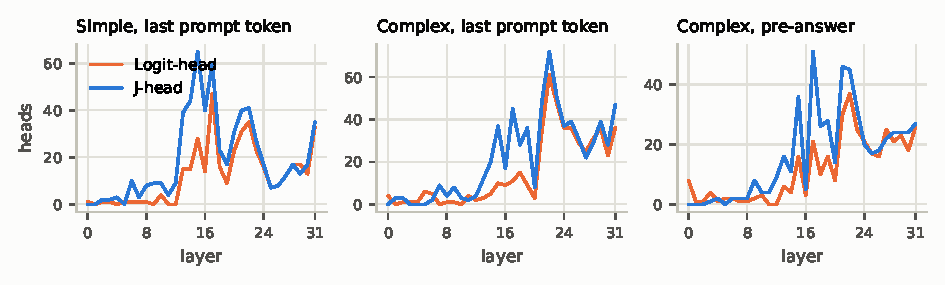
\includegraphics[width=\textwidth]{figures/layers.pdf}
\caption{Lexical task heads per layer under each readout, summed over the head sets of all tasks and styles, at the last prompt token. Left: simple tasks; right: complex tasks.}
\label{fig:layers}
\end{figure}

\begin{figure}[tbp]
\centering
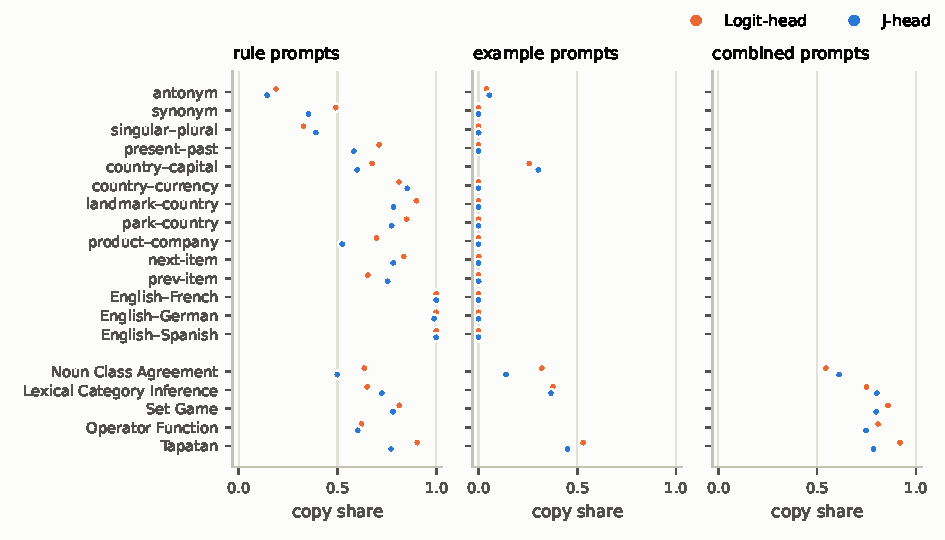
\includegraphics[width=\textwidth]{figures/copy_share.pdf}
\caption{Copy share of each head set (Sec.~\ref{sec:measures}): the share of prompts on which a head's matched terms occur in the prompt text, averaged over the set. Complex tasks at the last prompt token; missing points are empty sets.}
\label{fig:copy}
\end{figure}

\begin{figure}[p]
\centering
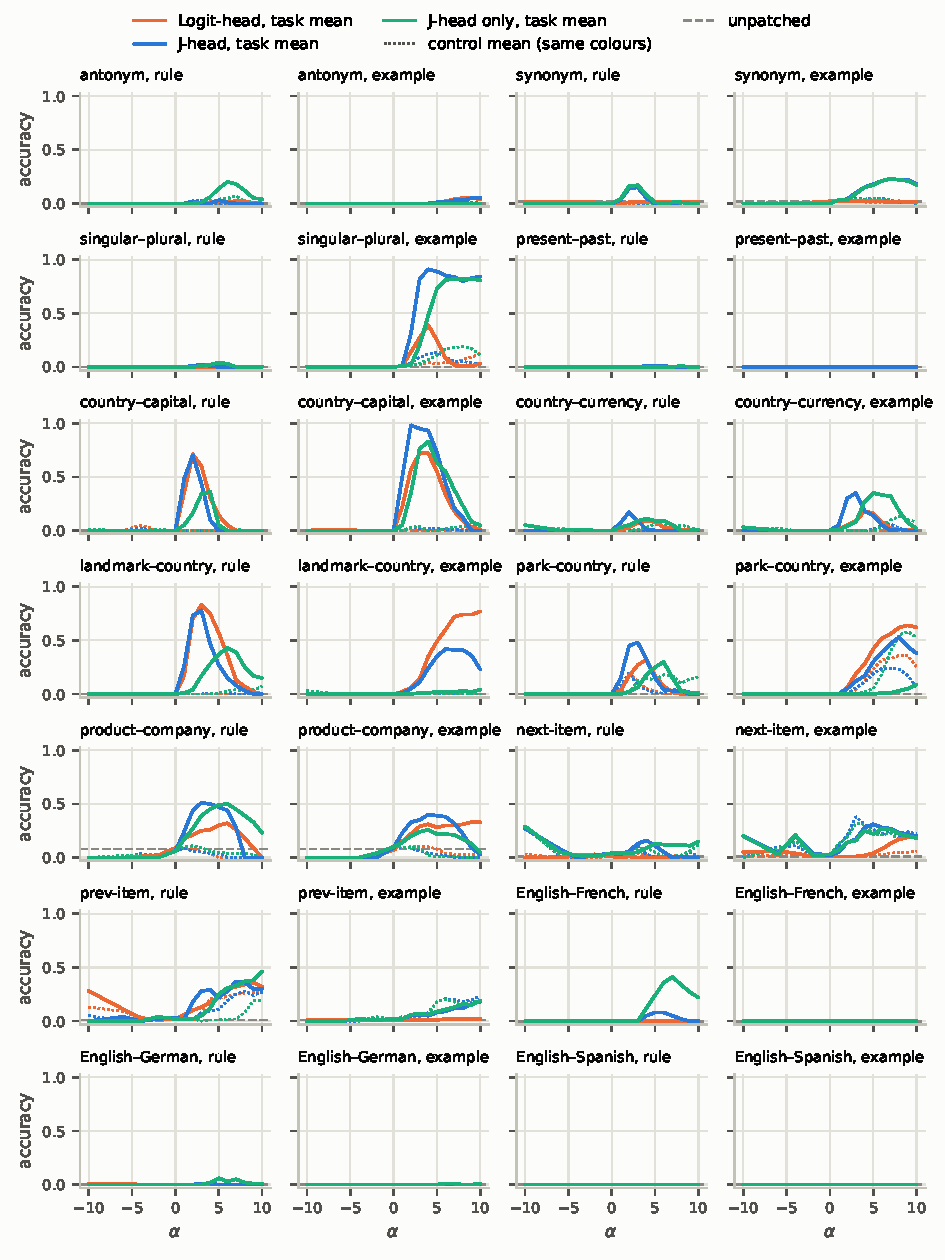
\includegraphics[width=\textwidth]{figures/patching_simple.pdf}
\caption{E1 causal check: accuracy on the 100 patched items of each task against $\alpha$, with each style's head set patched with means of the same style, averaged over the style's five source wordings. Solid: the head set's mean over the task's prompts; dotted: the control mean at the same heads; dashed: unpatched accuracy.}
\label{fig:patch-simple}
\end{figure}

\begin{figure}[p]
\centering
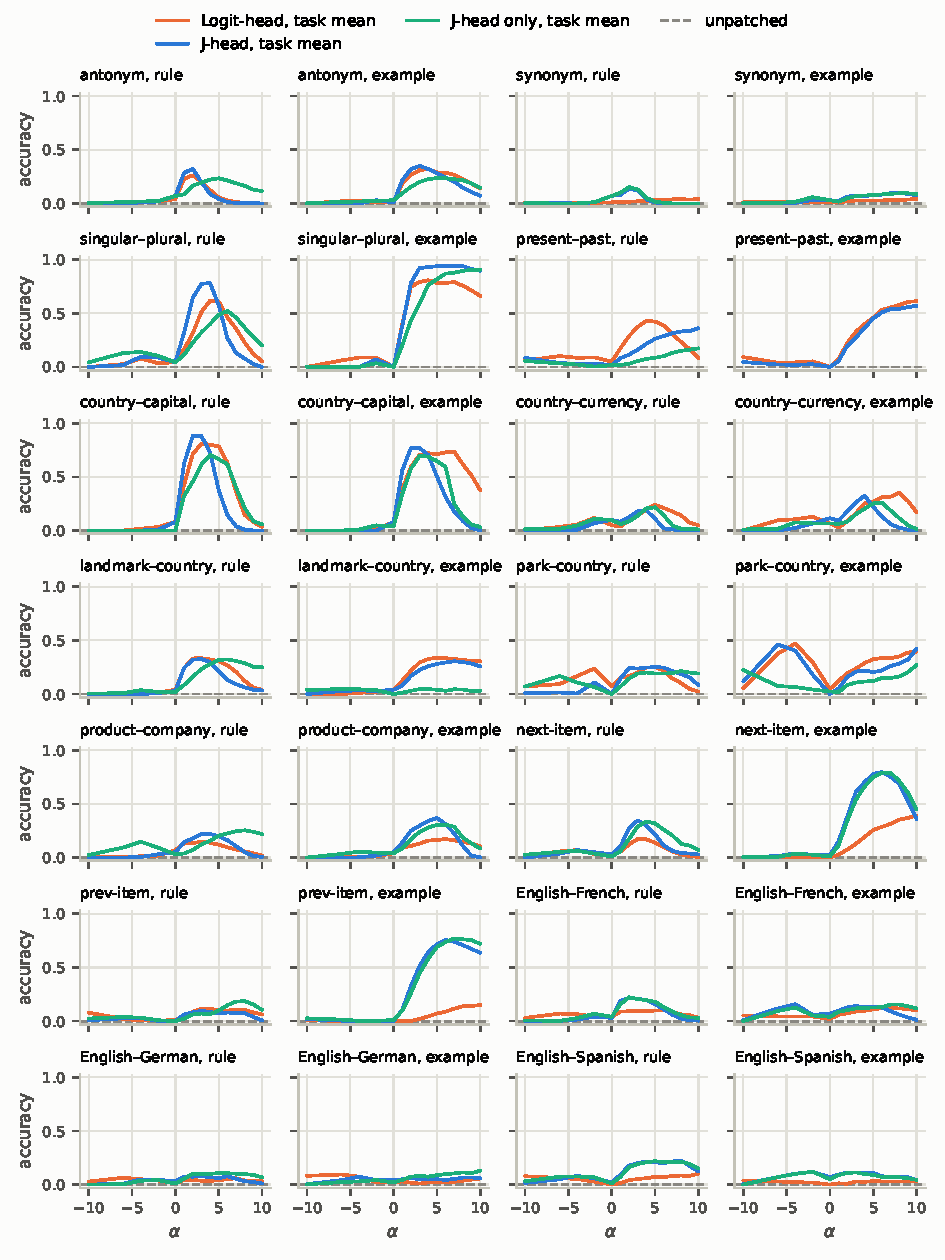
\includegraphics[width=\textwidth]{figures/patching_simple_wrong.pdf}
\caption{E1, second causal check, as Figure~\ref{fig:patch-simple}, with the wrongly answered 1-shot prompts patched. No control mean.}
\label{fig:patch-simple-wrong}
\end{figure}

\subsection{E2: Complex tasks}\label{sec:res-e2}
\paragraph{Head sets} (Table~\ref{tab:heads-complex}). Both readouts find lexical task heads for every complex task and style. The sets are larger than for the simple tasks, against H\ref{h:complex}, but the head counts of the two families are not comparable. The complex term lists expand to 114 to 340 token ids and the simple ones to 2 to 22, and a longer list makes a match among a head's ten top tokens more likely for any head. Small $P^{+}$ sets add to this: the example-style $P^{+}$ of Set Game is one prompt, so every head that matches on it is a lexical task head (9 and 13 heads), and for the example style of Operator Function (34 prompts) and of Tapatan (88) and Tapatan's combined style (47), 4 to 9 matching prompts suffice. As on the simple tasks, J-head finds more heads than Logit-head on every pair, and three fifths of its added heads lie in layers 10 to 19, while four fifths of the Logit-head heads lie in layer 20 or later. Its set covers 44\% to 91\% of the Logit-head set, never all of it. Of each example-style set, 48\% to 94\% is also in the rule-style set, at least half on 9 of the 10 pairs of task and readout (RQ3); the exception is Operator Function under J-head, and the example-style sets of Set Game rest on one prompt. Copy shares lie between about half and nine tenths under rule and combined prompts and are lower under example prompts: zero on Set Game and Operator Function, and above the near-zero values of the simple tasks' example prompts on the other three tasks (Figure~\ref{fig:copy}).

\paragraph{Causal check} (Tables~\ref{tab:effects-complex} and~\ref{tab:effects-complex-wrong}, Figure~\ref{fig:patch-complex}). In the first check, the prompts without task information get no answer on Noun Class Agreement, Lexical Category Inference, Operator Function and Tapatan: the model describes the input (a sentence in a coded language, items to classify, a board it takes for Sudoku or tic-tac-toe) or, on Operator Function, asks for the function. No patch changes this. Averaged over the seven means, accuracy stays at zero on the first three tasks, where some Operator Function replies box a number that is not the answer, and reaches at most two items on Tapatan, with task and control means alike; under any single mean and $\alpha$ it never exceeds three items. On Set Game, 58 of the 100 patched items are solved without task information, since the input block still asks which cards on the board form a set. Averaged over the seven means, the patches raise this by at most five items, and the control mean by as much or more. The first check shows no causal effect of the rule-style head sets on any complex task.

In the second check, every head set raises accuracy on the four tasks with wrongly answered items; Operator Function has none, since under the flexible score it answers every item correctly under its original rules prompt. The answers show that these gains need no task information. On Noun Class Agreement and Lexical Category Inference, the largest gains come where a patch makes the model give one label to (almost) every item. On Noun Class Agreement, the Logit-head set answers ``Yes'' to every item at $\alpha=10$ (0.58, the share of ``Yes'' among them) and ``No'' at $\alpha=-10$ (0.42); the J-head set answers ``No'' to every item at $\alpha$ of 4 and 6, and the heads found only by J-head from 6 to 10. On Lexical Category Inference, every set answers ``No'' to all items at $\alpha=4$ (0.28), and ``Yes'' to most at $\alpha=8$ (0.65 to 0.71, against 0.72 for answering ``Yes'' to all). No gain averaged over the seven means exceeds the accuracy of answering every item with one label. On Set Game and Tapatan, patches with no task content already fix part of the failures: setting the heads to zero ($\alpha=0$), or writing their own mean ($\alpha=1$), solves 21 to 23 of the 100 Set Game items and 13 to 17 of the Tapatan items. A change to the forward pass of the prompt gives the model another attempt at a problem it failed once, and it then solves some of them. At $\alpha=\pm10$ every set solves about half of the Set Game items (0.45 to 0.53); the model then writes a set almost at once (with the Logit-head set at $\alpha=10$, the median reply is 97 characters, against 868 at $\alpha=1$). Tapatan's gains stay below the share of its most frequent label among these items (0.43). Without a control mean, the second check cannot tell these gains apart from a patch that changes how the model answers, not what it computes.

\paragraph{Hypotheses.} For RQ1, the method finds lexical task heads for every complex task under both readouts, but neither check shows a task-specific effect for them: the first check changes nothing on four tasks and nothing beyond the control on Set Game, and the gains of the second check come with one label for every item or are matched in part by setting the heads to zero. This agrees with the causal part of H\ref{h:complex}; its head-count part cannot be tested with term lists of such different lengths. For H\ref{h:readout} on the complex tasks, both conditions fail: the J-head set misses part of the Logit-head set on every pair, and the heads found only by J-head have no task-specific effect. Together with E1, H\ref{h:readout} is falsified as stated, although on the simple tasks the heads that J-head adds have causal effects of their own.

\begin{table}[tbp]
\centering\footnotesize\setlength{\tabcolsep}{3.5pt}
% Generated by scripts/results_tex.py from results/.
\begin{tabular}{@{}lcccccccccccccc@{}}
\toprule
 & \multicolumn{4}{c}{Rule} & \multicolumn{4}{c}{Example} & \multicolumn{4}{c}{Combined} & \multicolumn{2}{c}{Rule $\cap$ ex.} \\
\cmidrule(lr){2-5}\cmidrule(lr){6-9}\cmidrule(lr){10-13}\cmidrule(lr){14-15}
Task & $|P^+|$ & L & J & L$\cap$J & $|P^+|$ & L & J & L$\cap$J & $|P^+|$ & L & J & L$\cap$J & L & J \\
\midrule
Noun Class Agreement & 100 & 18 & 22 & 10 & 100 & 12 & 17 & 6 & 100 & 22 & 35 & 17 & 8 & 10 \\
Lexical Category Inference & 100 & 39 & 51 & 31 & 100 & 16 & 22 & 10 & 73 & 46 & 61 & 39 & 13 & 15 \\
Set Game & 100 & 55 & 75 & 48 & 1 & 9 & 13 & 4 & 100 & 52 & 65 & 40 & 6 & 8 \\
\quad pre-answer & 100 & 54 & 62 & 42 & 1 & 12 & 21 & 6 & 100 & 56 & 72 & 46 & 8 & 9 \\
Operator Function & 100 & 24 & 41 & 20 & 1 & 9 & 14 & 6 & 100 & 22 & 38 & 20 & 5 & 10 \\
\quad pre-answer & 100 & 26 & 41 & 17 & 1 & 9 & 14 & 5 & 100 & 19 & 42 & 13 & 4 & 13 \\
Tapatan & 100 & 61 & 76 & 46 & 89 & 46 & 62 & 38 & 47 & 55 & 70 & 48 & 32 & 40 \\
\quad pre-answer & 100 & 69 & 94 & 52 & 89 & 70 & 112 & 58 & 47 & 85 & 112 & 67 & 44 & 64 \\
\bottomrule
\end{tabular}

\caption{E2: lexical task heads per task and style. $|P^{+}|$: identification prompts, the first (at most 100) answered correctly under the most accurate rule wording (rule; wording~6 for Noun Class Agreement and Lexical Category Inference, wording~5 for Set Game, the original prompt for Operator Function, whose seven wordings tie, wording~1 for Tapatan), under the example-based and under the combined prompts. L, J, L$\cap$J and Rule $\cap$ ex.\ as in Table~\ref{tab:heads-simple}.}
\label{tab:heads-complex}
\end{table}

\begin{table}[tbp]
\centering\footnotesize
% Generated by scripts/results_tex.py from results/.
\begin{tabular}{@{}lrccccccc@{}}
\toprule
 & & & \multicolumn{3}{c}{Task mean} & \multicolumn{3}{c}{Control mean} \\
\cmidrule(lr){4-6}\cmidrule(lr){7-9}
Task & Items & Baseline & L & J & J only & L & J & J only \\
\midrule
Noun Class Agreement & 100 & 0.00 & 0.00 & 0.00 & 0.00 & 0.00 & 0.00 & 0.00 \\
Lexical Category Inference & 100 & 0.00 & 0.00 & 0.00 & 0.00 & 0.00 & 0.00 & 0.00 \\
Set Game & 100 & 0.58 & 0.04 & 0.04 & 0.05 & 0.06 & 0.05 & 0.10 \\
Operator Function & 100 & 0.00 & 0.00 & 0.00 & 0.00 & 0.00 & 0.00 & 0.00 \\
Tapatan & 100 & 0.00 & 0.01 & 0.01 & 0.01 & 0.01 & 0.00 & 0.02 \\
\bottomrule
\end{tabular}

\caption{E2 causal check, as Table~\ref{tab:effects-simple}: the rule-style head sets, patched with the means of the seven rule wordings into the prompts without task information; accuracy is averaged over the seven means before the maximum is taken. Control mean: the control task's mean under its original rules prompt. 100 patched items per task, the 11 values of $\alpha$ of Sec.~\ref{sec:causal}.}
\label{tab:effects-complex}
\end{table}

\begin{table}[tbp]
\centering\footnotesize
% Generated by scripts/results_tex.py from results/.
\begin{tabular}{@{}lrccccccc@{}}
\toprule
 & & & \multicolumn{3}{c}{Task mean} & \multicolumn{3}{c}{Control mean} \\
\cmidrule(lr){4-6}\cmidrule(lr){7-9}
Task & Items & Baseline & L & J & J only & L & J & J only \\
\midrule
Noun Class Agreement & 100 & 0.00 & 0.58 & 0.44 & 0.46 & 0.42 & 0.80 & 0.59 \\
Lexical Category Inference & 100 & 0.00 & 0.71 & 0.65 & 0.71 & 0.72 & 0.72 & 0.72 \\
Set Game & 100 & 0.00 & 0.53 & 0.55 & 0.50 & 0.51 & 0.54 & 0.49 \\
Operator Function & \multicolumn{8}{l}{\textit{no item answered wrongly}} \\
Tapatan & 100 & 0.00 & 0.25 & 0.26 & 0.24 & 0.33 & 0.36 & 0.25 \\
\bottomrule
\end{tabular}

\caption{E2, second causal check, as Table~\ref{tab:effects-complex}, with the original rules prompts of the first 100 items answered wrongly under them patched; Operator Function answers every item correctly under its original rules prompt and has none. Unpatched accuracy is 0 by construction. No control mean. Answering every patched item with its more frequent label scores 0.58 on Noun Class Agreement and 0.72 on Lexical Category Inference (``Yes'' for both).}
\label{tab:effects-complex-wrong}
\end{table}

\begin{figure}[p]
\centering
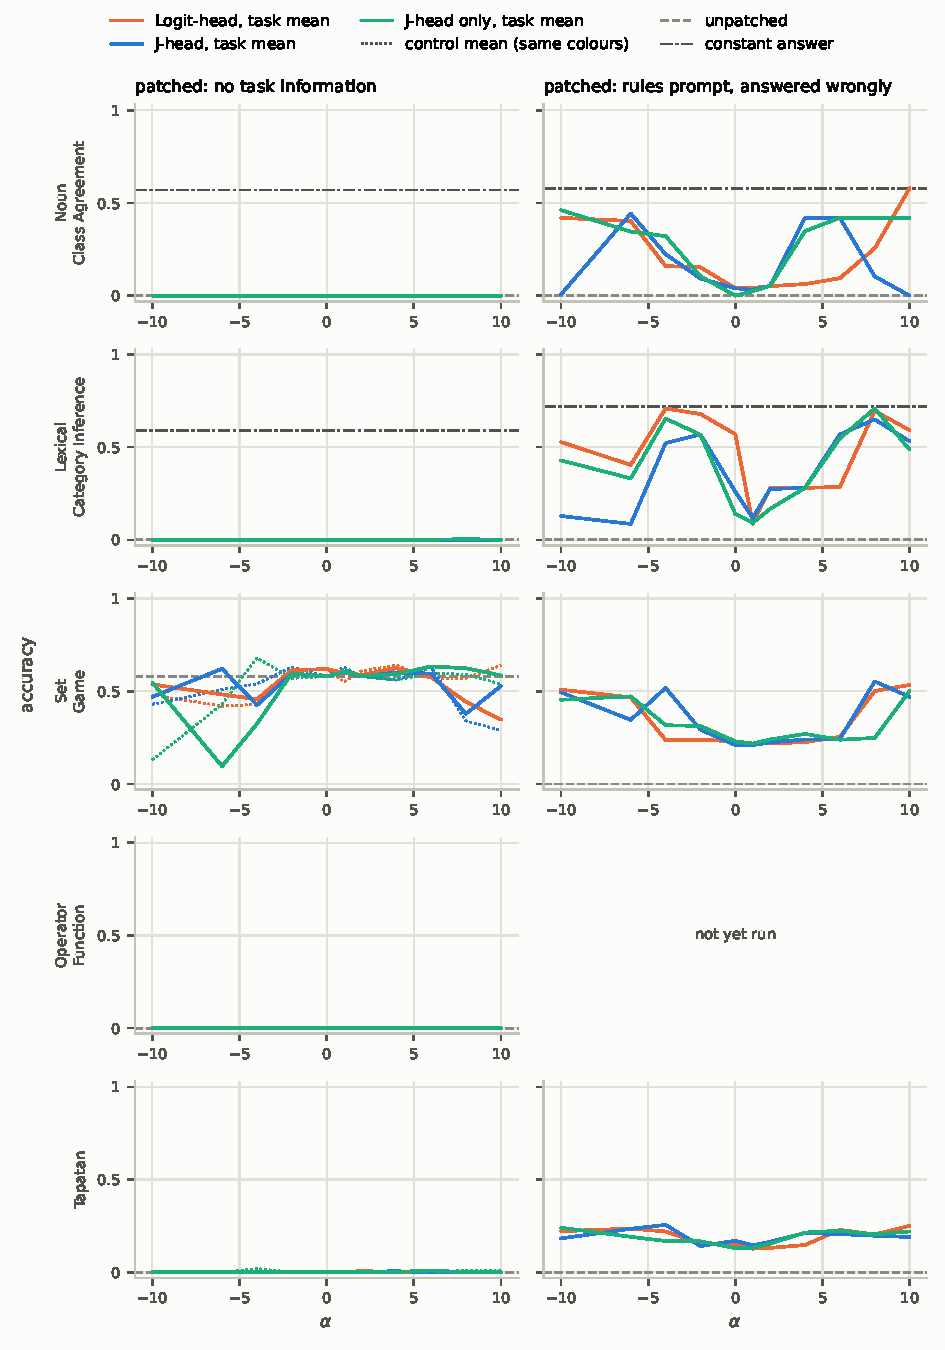
\includegraphics[width=\textwidth]{figures/patching_complex.pdf}
\caption{E2 causal checks, as Figure~\ref{fig:patch-simple}: the rule-style head sets, with accuracy averaged over the means of the seven rule wordings. Left: the prompts without task information patched (first check); right: the original rules prompts answered wrongly (second check, no control mean). 100 patched items per task; Operator Function has no second check. Constant answer: the accuracy of answering every patched item with its more frequent label.}
\label{fig:patch-complex}
\end{figure}

\section{Plan}\label{sec:plan}
\paragraph{Steps.}
\begin{enumerate}
\item Build the additions of Sec.~\ref{sec:adapt}: rule wordings (each checked to state the same rules as the original prompt), term lists, prompts without task information.
\item Run E0 and select tasks. Evaluate its saved outputs with the strict and the judged score (Sec.~\ref{sec:evaluation}).
\item Run E1.
\item Run E2.
\end{enumerate}
Reused code and data: the lexical-task-head code of \citet{yang2026shared}; the Head-JLens code and matrices of \citet{merlo2026headjlens}; the data and generation code of \citet{fu2026rules}; the task datasets of \citet{todd2024function}.

\paragraph{Limitations.} One model, and one difficulty level of each complex task. The term lists are generated by an LLM and checked by hand, and the identified heads depend on them. Rule-based prompts contain task words, so a head may decode them by copying from the prompt; the copy share measures this but does not decide it. Under J-head, some sites rank tokens highly on unrelated prompts as well \citep[Sec.~3.6]{merlo2026headjlens}, so a larger J-head set is not by itself evidence of more task representation; the causal check is needed. $P^{+}$ and the patched items are chosen by the flexible score, which accepts only the reference answer: a prompt answered with another valid answer is counted as wrong. The judged score depends on one LLM judge, which is not checked against hand labels here; \citet{hua2025flaw} find that LLM judges agree with human annotators on other tasks.

\paragraph{Deliverables.} Head sets, measures and causal-check curves for every task, style and readout.

\bibliographystyle{plainnat}
\bibliography{references}

\appendix

% Appendix: prompts and generated material for the complex tasks.
% Included from proposal-minimal.tex.

\section{Original rule prompts}\label{app:orig}
The rules-only prompts of \citet{fu2026rules}, from their released code (\url{https://github.com/tinlaboratory/rules-vs-examples}, \texttt{rules-mode-prompts/}, MIT licence). Text in curly braces is filled per item. Tapatan uses the final-board-state prompt, whose levels differ only in its parameters: board size 3, 5, 7 and line length 3, 4, 5 for Easy, Medium, Hard \citep[Table~1]{fu2026rules}; the version in \citet[App.~F]{fu2026rules} also states the maximum number of pieces per player and that at most one player has a winning line. The Medium and Hard prompts of Lexical Category Inference are identical within each logic variant.

\subsection*{Set Game}

\paragraph{Easy.}
\begin{promptbox}
You will be shown 9 cards on the board and have to select 3 cards that form a GAME-SET based on the following rules.

RULES:
1. Each card has two attributes: an animal and a biome.
2. There are 10 types of animals: armadillo, axolotl, bat, cat, fox, horse, rabbit, sheep, turtle, wolf.
3. There are 10 types of biomes: plain, savanna, desert, swamp, forest, jungle, taiga, hill, badland, tundra.
4. A GAME-SET is a set of three cards: For each attribute (animal, biome), the three cards must be either ALL the SAME or ALL DIFFERENT. e.g. if 2 of the cards have the same value, and 1 of them has a different value, the set is NOT valid.

Here is the board:

{board}

Based on the rules, tell me which three cards here constitute a GAME-SET. Type the cards in the following format:
 \boxed{First card: CARD1
Second card: CARD2
Third card: CARD3}
\end{promptbox}

\paragraph{Medium.}
\begin{promptbox}
You will be shown 9 cards on the board and have to select 3 cards that form a GAME-SET based on the following rules.

RULES:
1. Each card has three attributes: an animal, a biome, and a food.
2. There are 10 types of animals: armadillo, axolotl, bat, cat, fox, horse, rabbit, sheep, turtle, wolf.
3. There are 10 types of biomes: plain, savanna, desert, swamp, forest, jungle, taiga, hill, badland, tundra.
4. There are 10 types of food: apple, potato, bread, cake, carrot, mutton, beef, cookie, pie, melon.
5. A GAME-SET is a set of three cards: For each attribute (animal, biome, food), the three cards must be either ALL the SAME or ALL DIFFERENT. e.g. if 2 of the cards have the same value, and 1 of them has a different value, the set is NOT valid.

Here is the board:

{board}

Based on the rules, tell me which three cards here constitute a GAME-SET. Type the cards in the following format:
 \boxed{First card: CARD1
Second card: CARD2
Third card: CARD3}
\end{promptbox}

\paragraph{Hard.}
\begin{promptbox}
You will be shown 9 cards on the board and have to select 3 cards that form a GAME-SET based on the following rules.

RULES:
1. Each card has a number and three attributes: an animal, a biome, and a food.
2. Numbers range from 1 to 12.
3. There are 10 types of animals: armadillo, axolotl, bat, cat, fox, horse, rabbit, sheep, turtle, wolf.
4. There are 10 types of biomes: plain, savanna, desert, swamp, forest, jungle, taiga, hill, badland, tundra.
5. There are 10 types of food: apple, potato, bread, cake, carrot, mutton, beef, cookie, pie, melon.
6. A GAME-SET is a set of three cards: For each attribute (animal, biome, food), the three cards must be either ALL the SAME or ALL DIFFERENT. e.g. if 2 of the cards have the same value, and 1 of them has a different value, the set is NOT valid.
7. But only for the number, 2 of the cards should have the same number, and 1 of them should have a different number in order for the set to be valid.

Here is the board:

{board}

Based on the rules, tell me which three cards here constitute a GAME-SET. Type the cards in the following format:
 \boxed{First card: CARD1
Second card: CARD2
Third card: CARD3}
\end{promptbox}

\subsection*{Tapatan}

\paragraph{all levels.}
\begin{promptbox}
You will be learning a new board game. You will then be given one final board state from that game. Determine the current game outcome.

RULES:
1. The board is a {board_size}x{board_size} grid of points with coordinates (x,y), where 0 <= x,y < {board_size}.
2. A board cell contains A for player A's piece, B for player B's piece, or . for an empty point.
3. Orthogonal neighbors are always adjacent. Diagonal neighbors are adjacent only from even-parity points where (x+y) is even: (x,y) connects to (x±1,y±1) when in bounds.
4. A player wins if they have {line_length} pieces in a straight line (horizontal, vertical, or diagonal) and each consecutive pair of points in that line is adjacent under rule 3.
5. If A has a valid winning line, output A win. If B has a valid winning line, output B win. If neither player has a valid winning line, output continue.
6. You must output a label that is exactly one of: A win, B win, or continue.

BOARD:
{board_state}

LABEL:
\end{promptbox}

\subsection*{Operator Function}

\paragraph{Easy.}
\begin{promptbox}
You will be shown a problem that uses a newly defined operator function based on the following rules and need to calculate the answer for the problem.

RULES:
1. The new operator function f is composed of two arithmetic operators, and its inputs are integers.
2. Let x, y, z be inputs of the function.
3. To compute f(x,y,z), first multiply x and y.
4. Then, add z to the result from the previous operation.
Problem: \({problem}\)
Answer (place the result in \boxed{}):\boxed{}
\end{promptbox}

\paragraph{Medium.}
\begin{promptbox}
You will be shown a problem that uses a newly defined operator function based on the following rules and need to calculate the answer for the problem.

RULES:
1. The new operator function g is composed of three arithmetic operators, and its inputs are integers.
2. Let x, y, z, a be inputs of the function.
3. To compute g(x,y,z,a), first subtract y from x.
4. Second, multiply the result from the previous operation by z.
5. Last, adds a to the result of the previous operation.
Problem: \({problem}\)
Answer (place the result in \boxed{}):\boxed{}
\end{promptbox}

\paragraph{Hard.}
\begin{promptbox}
You will be shown a problem that uses a newly defined operator function based on the following rules and need to calculate the answer for the problem.

RULES:
1. The new operator function h is composed of four arithmetic operators, and its inputs are integers.
2. Let x, y, z, a, b be inputs of the function.
3. To compute h(x,y,z,a,b), first add x and y.
4. Second, multiply the result from the previous operation by z.
5. Third, subtract a from the result of the previous operation.
6. Last, take the remainder when the result is divided by b.
Problem: \({problem}\)
Answer (place the result in \boxed{}):\boxed{}
\end{promptbox}

\subsection*{Noun Class Agreement}

\paragraph{Easy.}
\begin{promptbox}
You will be given one sentence in a synthetic language. Decide whether the sentence is grammatical.

RULES:
1. There are 2 noun classes: A and B.
2. Each noun phrase has the form DET NOUN.
3. The class A determiner is ka, and the class B determiner is ti.
4. The class A nouns are tac, sular, fep, wug. The class B nouns are bim, noko, glarn, zesh.
5. Sentences follow the template DET NOUN VERB DET NOUN.
6. Verbs are plain roots like dax, miv, lorp and never change.
7. A sentence is grammatical if and only if, in each noun phrase, the determiner matches the noun's class.
8. Your answer must be exactly one word: Yes or No.

Sentence: {sentence}
Answer:
\end{promptbox}

\paragraph{Medium.}
\begin{promptbox}
You will be given one sentence in a synthetic language. Decide whether the sentence is grammatical.

RULES:
1. There are 4 noun classes: A, B, C, D.
2. A noun phrase has the form DET ADJ-SUFF NOUN.
3. The class A determiner is ka, the class B determiner is ti, the class C determiner is su, and the class D determiner is vo.
4. Adjectives have the form STEM-SUFFIX. The suffix must match the noun's class.
5. The class A adjective suffix is -en, the class B adjective suffix is -os, the class C adjective suffix is -im, and the class D adjective suffix is -at.
6. Example adjective tokens are glim-en, prun-os, fen-im, zay-at.
7. The class A nouns are tav, fap. The class B nouns are bim, glarn. The class C nouns are sular, wug. The class D nouns are noko, zesh.
8. Sentences follow the template DET ADJ-SUFF NOUN VERB DET ADJ-SUFF NOUN.
9. Verbs are plain roots like dax, miv, lorp and never change.
10. A sentence is grammatical if and only if, in each noun phrase, both the determiner and the adjective suffix match the noun's class.
11. Your answer must be exactly one word: Yes or No.

Sentence: {sentence}
Answer:
\end{promptbox}

\paragraph{Hard.}
\begin{promptbox}
You will be given one sentence in a synthetic language. Decide whether the sentence is grammatical.

RULES:
1. There are 6 noun classes: A, B, C, D, E, F.
2. A noun phrase has the form DET ADJ-SUFF NOUN.
3. The class A determiner is ka, the class B determiner is ti, the class C determiner is su, the class D determiner is vo, the class E determiner is ne, and the class F determiner is la.
4. Adjectives have the form STEM-SUFFIX. The suffix must match the noun's class.
5. The class A adjective suffix is -en, the class B adjective suffix is -os, the class C adjective suffix is -im, the class D adjective suffix is -at, the class E adjective suffix is -uk, and the class F adjective suffix is -esh.
6. The verb has the form PREFIX-ROOT-SUFFIX.
7. The prefix must match the class of the subject noun, and the suffix must match the class of the object noun.
8. The class A subject prefix is ge-, the class B subject prefix is du-, the class C subject prefix is ri-, the class D subject prefix is zo-, the class E subject prefix is pa-, and the class F subject prefix is li-.
9. The class A object suffix is -an, the class B object suffix is -eb, the class C object suffix is -ig, the class D object suffix is -ot, the class E object suffix is -ul, and the class F object suffix is -er.
10. Example verb tokens are ge-dax-eb, pa-miv-ig, du-lorp-er.
11. The class A nouns are tav, fap. The class B nouns are bim, glarn. The class C nouns are sular, wug. The class D nouns are noko, zesh. The class E nouns are tac, fep. The class F nouns are lurn, prax.
12. Sentences follow the template DET ADJ-SUFF NOUN PREFIX-ROOT-SUFFIX DET ADJ-SUFF NOUN.
13. Verb roots are plain roots like dax, miv, lorp. Only the verb's prefix and suffix change.
14. A sentence is grammatical if and only if the subject noun phrase's determiner and adjective suffix match the subject noun's class, the object noun phrase's determiner and adjective suffix match the object noun's class, the verb prefix matches the subject noun's class, and the verb suffix matches the object noun's class.
15. Your answer must be exactly one word: Yes or No.

Sentence: {sentence}
Answer:
\end{promptbox}

\subsection*{Lexical Category Inference}

\paragraph{Easy.}
\begin{promptbox}
You will be shown a list of four words. Decide whether this list is correct based on the following rules.

RULES:
1. There are exactly four categories: {prompt_labels}.
2. Each category has the meaning shown in the category definitions below.
3. A correct list contains exactly four comma-separated items.
4. In a correct list, the first item is a member of Category 1, the second item is a member of Category 2, and so on.
5. If a category says "at least one", an item may satisfy any listed description. If it says "all", an item must satisfy every listed description.
6. Your answer must be exactly one word: Yes or No.

CATEGORY DEFINITIONS:
{label_block}

List: {candidate_block}
Answer:
\end{promptbox}

\paragraph{Medium and Hard, OR.}
\begin{promptbox}
You will be shown a list of four words. Decide whether this list is correct based on the following rules.

RULES:
1. There are exactly four categories: {prompt_labels}.
2. Each category has the meaning shown in the category definitions below.
3. A correct list contains exactly four comma-separated items.
4. In a correct list, the first item is a member of Category 1, the second item is a member of Category 2, and so on.
5. If a category lists multiple descriptions, an item is a member of that category if it satisfies at least one listed description.
6. Your answer must be exactly one word: Yes or No.

CATEGORY DEFINITIONS:
{label_block}

List: {candidate_block}
Answer:
\end{promptbox}

\paragraph{Medium and Hard, AND.}
\begin{promptbox}
You will be shown a list of four words. Decide whether this list is correct based on the following rules.

RULES:
1. There are exactly four categories: {prompt_labels}.
2. Each category has the meaning shown in the category definitions below.
3. A correct list contains exactly four comma-separated items.
4. In a correct list, the first item is a member of Category 1, the second item is a member of Category 2, and so on.
5. If a category lists multiple descriptions, an item is a member of that category only if it satisfies all listed descriptions.
6. Your answer must be exactly one word: Yes or No.

CATEGORY DEFINITIONS:
{label_block}

List: {candidate_block}
Answer:
\end{promptbox}

\section{Generation prompts}\label{app:genprompts}
Both prompts are given to GPT-5.5 through the Azure OpenAI API; \texttt{\{rule\_prompt\}} is an original prompt of App.~\ref{app:orig}.

\subsection*{Rule wordings}
\begin{promptbox}
You will be given a prompt that describes the rules of a task for a language model. Write {N} paraphrases of it.

Requirements:
1. Each paraphrase must state exactly the same rules as the original: the same constraints, conditions, quantities, names, symbols and labels. Do not add, remove, weaken or strengthen any rule, and do not add examples, hints or explanations.
2. Change the wording and the sentence structure. Reorder rules only where their order does not matter; if a rule refers to another rule by its number, keep the reference correct.
3. Copy verbatim every placeholder in curly braces (e.g. {board}), the answer-format instruction, and every output label or format string (e.g. "Yes or No", "A win, B win, or continue", \boxed{...}).
4. Keep unchanged the final lines that introduce the input and the answer (e.g. "Sentence: {sentence}" and "Answer:").
5. The paraphrases must differ from the original and from each other.

Return a JSON list of {N} strings.

Original prompt:
<<<
{rule_prompt}
>>>
\end{promptbox}

\subsection*{Term lists}
\begin{promptbox}
You will be given the rules of a task for a language model. List words that describe the task itself: what the task asks the model to do, its operation or relation, and its key concepts. For example, for the task "give the antonym of a word": opposite, reverse, antonym, contrary.

Requirements:
1. Single words only.
2. Do not list possible answers or output labels, words that only name the items of a particular input (e.g. specific animals, nouns or numbers), or placeholders.
3. Include singular and plural forms and capitalised forms. You may include translations into other languages.
4. Return a JSON list of strings.

Task rules:
<<<
{rule_prompt}
>>>
\end{promptbox}

\section{Rule wordings}\label{app:wordings}
The six wordings of each original rules prompt of App.~\ref{app:orig} at the easy level, the level in the study, generated and checked as in Sec.~\ref{sec:adapt}. Text in curly braces is filled per item.

% Generated by scripts/appendix_tex.py from materials/complex/wordings.json.

\subsection*{Set Game, easy level}

\paragraph{Wording 1.}
\begin{promptbox}
You will see 9 cards on the board, and your task is to choose 3 cards that make a GAME-SET according to these rules.

RULES:
1. Every card has two attributes: an animal and a biome.
2. The 10 animal types are: armadillo, axolotl, bat, cat, fox, horse, rabbit, sheep, turtle, wolf.
3. The 10 biome types are: plain, savanna, desert, swamp, forest, jungle, taiga, hill, badland, tundra.
4. A GAME-SET consists of three cards: For each attribute (animal, biome), the values across the three cards must be either ALL the SAME or ALL DIFFERENT. For example, if 2 cards share the same value and 1 card has a different value, the set is NOT valid.

Here is the board:

{board}

Based on the rules, tell me which three cards here constitute a GAME-SET. Type the cards in the following format:
 \boxed{First card: CARD1
Second card: CARD2
Third card: CARD3}
\end{promptbox}

\paragraph{Wording 2.}
\begin{promptbox}
You are given a board with 9 cards and must pick 3 cards that constitute a GAME-SET under the rules below.

RULES:
1. Each card contains two attributes: an animal and a biome.
2. The animals come in 10 types: armadillo, axolotl, bat, cat, fox, horse, rabbit, sheep, turtle, wolf.
3. The biomes come in 10 types: plain, savanna, desert, swamp, forest, jungle, taiga, hill, badland, tundra.
4. A GAME-SET is a set of three cards: For each attribute (animal, biome), the three cards must have values that are either ALL the SAME or ALL DIFFERENT. For instance, when 2 cards have the same value and 1 card has another value, the set is NOT valid.

Here is the board:

{board}

Based on the rules, tell me which three cards here constitute a GAME-SET. Type the cards in the following format:
 \boxed{First card: CARD1
Second card: CARD2
Third card: CARD3}
\end{promptbox}

\paragraph{Wording 3.}
\begin{promptbox}
A board containing 9 cards will be shown, and you need to select 3 cards that form a GAME-SET by following the rules.

RULES:
1. Each card is defined by two attributes: an animal and a biome.
2. There are 10 animal types: armadillo, axolotl, bat, cat, fox, horse, rabbit, sheep, turtle, wolf.
3. There are 10 biome types: plain, savanna, desert, swamp, forest, jungle, taiga, hill, badland, tundra.
4. A GAME-SET is made up of three cards: For each attribute (animal, biome), the three cards must be either ALL the SAME or ALL DIFFERENT. If, for example, 2 of the cards have one value and 1 has a different value, the set is NOT valid.

Here is the board:

{board}

Based on the rules, tell me which three cards here constitute a GAME-SET. Type the cards in the following format:
 \boxed{First card: CARD1
Second card: CARD2
Third card: CARD3}
\end{promptbox}

\paragraph{Wording 4.}
\begin{promptbox}
You will be presented with 9 cards on the board and must identify 3 cards that create a GAME-SET according to the following rules.

RULES:
1. Each card has two attributes: an animal and a biome.
2. The 10 kinds of animals are: armadillo, axolotl, bat, cat, fox, horse, rabbit, sheep, turtle, wolf.
3. The 10 kinds of biomes are: plain, savanna, desert, swamp, forest, jungle, taiga, hill, badland, tundra.
4. A GAME-SET is a group of three cards: For each attribute (animal, biome), the three cards must be either ALL the SAME or ALL DIFFERENT. e.g. when 2 of the cards share the same value and 1 of them has a different value, the set is NOT valid.

Here is the board:

{board}

Based on the rules, tell me which three cards here constitute a GAME-SET. Type the cards in the following format:
 \boxed{First card: CARD1
Second card: CARD2
Third card: CARD3}
\end{promptbox}

\paragraph{Wording 5.}
\begin{promptbox}
From the 9 cards displayed on the board, choose 3 cards that satisfy the definition of a GAME-SET using these rules.

RULES:
1. Each card includes two attributes: an animal and a biome.
2. There are 10 types of animals: armadillo, axolotl, bat, cat, fox, horse, rabbit, sheep, turtle, wolf.
3. There are 10 types of biomes: plain, savanna, desert, swamp, forest, jungle, taiga, hill, badland, tundra.
4. A GAME-SET is a collection of three cards: For each attribute (animal, biome), the three cards must be either ALL the SAME or ALL DIFFERENT. e.g. if 2 of the cards have the same value while 1 of them has a different value, the set is NOT valid.

Here is the board:

{board}

Based on the rules, tell me which three cards here constitute a GAME-SET. Type the cards in the following format:
 \boxed{First card: CARD1
Second card: CARD2
Third card: CARD3}
\end{promptbox}

\paragraph{Wording 6.}
\begin{promptbox}
You will be shown a board of 9 cards, and you have to determine 3 cards that form a GAME-SET based on the rules below.

RULES:
1. Each card has two attributes: an animal and a biome.
2. The animal attribute has 10 possible types: armadillo, axolotl, bat, cat, fox, horse, rabbit, sheep, turtle, wolf.
3. The biome attribute has 10 possible types: plain, savanna, desert, swamp, forest, jungle, taiga, hill, badland, tundra.
4. A GAME-SET is a set containing three cards: For each attribute (animal, biome), the three cards must be either ALL the SAME or ALL DIFFERENT. e.g. if 2 of the cards have matching values and 1 of them has a different value, the set is NOT valid.

Here is the board:

{board}

Based on the rules, tell me which three cards here constitute a GAME-SET. Type the cards in the following format:
 \boxed{First card: CARD1
Second card: CARD2
Third card: CARD3}
\end{promptbox}

\subsection*{Operator Function, easy level}

\paragraph{Wording 1.}
\begin{promptbox}
A problem involving a newly defined operator function will be presented, and you must determine its answer using these rules.

RULES:
1. The new operator function f consists of two arithmetic operators, and all of its inputs are integers.
2. Let x, y, z be the inputs to the function.
3. When computing f(x,y,z), begin by multiplying x and y.
4. After that, add z to the outcome of the preceding operation.
Problem: \({problem}\)
Answer (place the result in \boxed{}):\boxed{}
\end{promptbox}

\paragraph{Wording 2.}
\begin{promptbox}
You need to solve a problem that uses a newly introduced operator function defined according to the rules below.

RULES:
1. The new operator function f is made from two arithmetic operators, and its inputs are integers.
2. Let x, y, z represent the inputs of the function.
3. To evaluate f(x,y,z), multiply x by y first.
4. Next, add z to the result obtained from the previous operation.
Problem: \({problem}\)
Answer (place the result in \boxed{}):\boxed{}
\end{promptbox}

\paragraph{Wording 3.}
\begin{promptbox}
A problem will be given that relies on a newly defined operator function; compute the answer by applying the following rules.

RULES:
1. The new operator function f is formed using two arithmetic operators, and the inputs to it are integers.
2. Let x, y, z be inputs of the function.
3. For f(x,y,z), first take the product of x and y.
4. Then add z to the result of that prior operation.
Problem: \({problem}\)
Answer (place the result in \boxed{}):\boxed{}
\end{promptbox}

\paragraph{Wording 4.}
\begin{promptbox}
You will receive a problem using a newly defined operator function, and you must calculate the result according to these rules.

RULES:
1. The new operator function f is built from two arithmetic operators, and its inputs are integers.
2. Let x, y, z denote the inputs of the function.
3. In computing f(x,y,z), the first step is to multiply x and y.
4. The next step is to add z to the result from the previous operation.
Problem: \({problem}\)
Answer (place the result in \boxed{}):\boxed{}
\end{promptbox}

\paragraph{Wording 5.}
\begin{promptbox}
The problem shown will involve a newly defined operator function, and the answer must be found using the rules that follow.

RULES:
1. The new operator function f is composed of two arithmetic operators, with integer inputs.
2. Let x, y, z be the function's inputs.
3. To calculate f(x,y,z), start by multiplying x and y.
4. Then add z to the value produced by the preceding operation.
Problem: \({problem}\)
Answer (place the result in \boxed{}):\boxed{}
\end{promptbox}

\paragraph{Wording 6.}
\begin{promptbox}
Use the rules below to calculate the answer to a problem involving a newly defined operator function.

RULES:
1. The new operator function f contains two arithmetic operators, and the inputs are integers.
2. Let x, y, z be inputs of the function.
3. To compute f(x,y,z), multiply x and y before anything else.
4. Then add z to the result from the previous operation.
Problem: \({problem}\)
Answer (place the result in \boxed{}):\boxed{}
\end{promptbox}

\subsection*{Noun Class Agreement, easy level}

\paragraph{Wording 1.}
\begin{promptbox}
You will receive a single sentence in a synthetic language. Determine whether it is grammatical.

RULES:
1. The language has 2 noun classes: A and B.
2. Every noun phrase is structured as DET NOUN.
3. ka is the determiner for class A, and ti is the determiner for class B.
4. The nouns in class A are tac, sular, fep, wug. The nouns in class B are bim, noko, glarn, zesh.
5. Sentences use the pattern DET NOUN VERB DET NOUN.
6. The verbs are plain roots like dax, miv, lorp and never change.
7. A sentence is grammatical exactly when, in every noun phrase, the determiner matches the noun's class.
8. Your answer must be exactly one word: Yes or No.

Sentence: {sentence}
Answer:
\end{promptbox}

\paragraph{Wording 2.}
\begin{promptbox}
You will be provided with one sentence written in a synthetic language. Judge whether the sentence is grammatical.

RULES:
1. There are 2 noun classes: A and B.
2. A noun phrase always has the form DET NOUN.
3. The determiner for class A is ka, and the determiner for class B is ti.
4. Class A contains the nouns tac, sular, fep, wug. Class B contains the nouns bim, noko, glarn, zesh.
5. A sentence follows the template DET NOUN VERB DET NOUN.
6. Verbs are plain roots like dax, miv, lorp and never change.
7. A sentence is grammatical if and only if the determiner in each noun phrase matches the noun's class.
8. Your answer must be exactly one word: Yes or No.

Sentence: {sentence}
Answer:
\end{promptbox}

\paragraph{Wording 3.}
\begin{promptbox}
You will see one sentence in a synthetic language. Decide if that sentence is grammatical.

RULES:
1. The noun classes are 2 in number: A and B.
2. Each noun phrase is of the form DET NOUN.
3. ka is used as the class A determiner, and ti is used as the class B determiner.
4. tac, sular, fep, wug are the class A nouns. bim, noko, glarn, zesh are the class B nouns.
5. Sentences have the template DET NOUN VERB DET NOUN.
6. Verbs are plain roots like dax, miv, lorp and never change.
7. A sentence is grammatical if and only if each noun phrase has a determiner that matches the noun's class.
8. Your answer must be exactly one word: Yes or No.

Sentence: {sentence}
Answer:
\end{promptbox}

\paragraph{Wording 4.}
\begin{promptbox}
A single sentence in a synthetic language will be given to you. Decide whether it is grammatical.

RULES:
1. There are 2 noun classes, A and B.
2. Noun phrases take the form DET NOUN.
3. The class A determiner is ka; the class B determiner is ti.
4. The class A nouns are tac, sular, fep, wug. The class B nouns are bim, noko, glarn, zesh.
5. Sentences are built according to DET NOUN VERB DET NOUN.
6. Verbs are plain roots like dax, miv, lorp and never change.
7. A sentence is grammatical if and only if, for each noun phrase, the determiner matches the noun's class.
8. Your answer must be exactly one word: Yes or No.

Sentence: {sentence}
Answer:
\end{promptbox}

\paragraph{Wording 5.}
\begin{promptbox}
You will get one sentence from a synthetic language. Determine whether the sentence is grammatical.

RULES:
1. There are 2 noun classes: A and B.
2. The form of every noun phrase is DET NOUN.
3. For class A, the determiner is ka, and for class B, the determiner is ti.
4. The class A nouns are tac, sular, fep, wug. The class B nouns are bim, noko, glarn, zesh.
5. Sentences conform to the template DET NOUN VERB DET NOUN.
6. Verbs are plain roots like dax, miv, lorp and never change.
7. A sentence is grammatical if and only if the determiner matches the noun's class in each noun phrase.
8. Your answer must be exactly one word: Yes or No.

Sentence: {sentence}
Answer:
\end{promptbox}

\paragraph{Wording 6.}
\begin{promptbox}
You will be shown one sentence in a synthetic language. Decide whether that sentence is grammatical.

RULES:
1. The language includes 2 noun classes: A and B.
2. Each noun phrase follows the form DET NOUN.
3. ka is the class A determiner, while ti is the class B determiner.
4. The class A nouns are tac, sular, fep, wug. The class B nouns are bim, noko, glarn, zesh.
5. Sentences follow this template: DET NOUN VERB DET NOUN.
6. Verbs are plain roots like dax, miv, lorp and never change.
7. A sentence is grammatical if and only if, within every noun phrase, the determiner matches the noun's class.
8. Your answer must be exactly one word: Yes or No.

Sentence: {sentence}
Answer:
\end{promptbox}

\subsection*{Tapatan, easy level}

\paragraph{Wording 1.}
\begin{promptbox}
You are going to learn a new board game. After that, you will receive a single final board state from the game. Decide the present game outcome.

RULES:
1. The board is a {board_size}x{board_size} grid of points whose coordinates are (x,y), with 0 <= x,y < {board_size}.
2. Each board cell holds A for player A's piece, B for player B's piece, or . for an empty point.
3. Orthogonal neighbors are always adjacent. Diagonal neighbors are adjacent only from even-parity points where (x+y) is even: (x,y) connects to (x±1,y±1) when in bounds.
4. A player wins when they have {line_length} pieces in one straight line (horizontal, vertical, or diagonal), with every consecutive pair of points in that line adjacent according to rule 3.
5. If A has a valid winning line, output A win. If B has a valid winning line, output B win. If neither player has a valid winning line, output continue.
6. You must output a label that is exactly one of: A win, B win, or continue.

BOARD:
{board_state}

LABEL:
\end{promptbox}

\paragraph{Wording 2.}
\begin{promptbox}
You will be taught a new board game, and then you will be shown one final board state from that game. Identify the game outcome at that moment.

RULES:
1. The board consists of a {board_size}x{board_size} grid of points at coordinates (x,y), where 0 <= x,y < {board_size}.
2. A board cell contains A for player A's piece, B for player B's piece, or . for an empty point.
3. Orthogonal neighbors are always adjacent. Diagonal neighbors are adjacent only from even-parity points where (x+y) is even: (x,y) connects to (x±1,y±1) when in bounds.
4. A player wins if they possess {line_length} pieces in a straight line (horizontal, vertical, or diagonal) and each successive pair of points in that line is adjacent under rule 3.
5. If A has a valid winning line, output A win. If B has a valid winning line, output B win. If neither player has a valid winning line, output continue.
6. You must output a label that is exactly one of: A win, B win, or continue.

BOARD:
{board_state}

LABEL:
\end{promptbox}

\paragraph{Wording 3.}
\begin{promptbox}
You will learn the rules for a new board game. You will then be provided with one final board state from it. Determine what the current outcome of the game is.

RULES:
1. The board is a grid of points with size {board_size}x{board_size} and coordinates (x,y), where 0 <= x,y < {board_size}.
2. In a board cell, A denotes player A's piece, B denotes player B's piece, and . denotes an empty point.
3. Orthogonal neighbors are always adjacent. Diagonal neighbors are adjacent only from even-parity points where (x+y) is even: (x,y) connects to (x±1,y±1) when in bounds.
4. A player wins by having {line_length} pieces in a straight line (horizontal, vertical, or diagonal), provided that each consecutive pair of points in that line is adjacent under rule 3.
5. If A has a valid winning line, output A win. If B has a valid winning line, output B win. If neither player has a valid winning line, output continue.
6. You must output a label that is exactly one of: A win, B win, or continue.

BOARD:
{board_state}

LABEL:
\end{promptbox}

\paragraph{Wording 4.}
\begin{promptbox}
You will be introduced to a new board game. Next, one final board state from the game will be given to you. Work out the current game outcome.

RULES:
1. The board is a {board_size}x{board_size} grid made of points with coordinates (x,y), where 0 <= x,y < {board_size}.
2. A board cell contains A for player A's piece, B for player B's piece, or . for an empty point.
3. Orthogonal neighbors are always adjacent. Diagonal neighbors are adjacent only from even-parity points where (x+y) is even: (x,y) connects to (x±1,y±1) when in bounds.
4. A player wins if {line_length} of their pieces form a straight line (horizontal, vertical, or diagonal) and every consecutive pair of points in that line is adjacent under rule 3.
5. If A has a valid winning line, output A win. If B has a valid winning line, output B win. If neither player has a valid winning line, output continue.
6. You must output a label that is exactly one of: A win, B win, or continue.

BOARD:
{board_state}

LABEL:
\end{promptbox}

\paragraph{Wording 5.}
\begin{promptbox}
You will receive the rules of a new board game. Then you will be given one final state of the board from that game. Determine the outcome currently shown.

RULES:
1. The board is a {board_size}x{board_size} point grid using coordinates (x,y), where 0 <= x,y < {board_size}.
2. A board cell contains A for player A's piece, B for player B's piece, or . for an empty point.
3. Orthogonal neighbors are always adjacent. Diagonal neighbors are adjacent only from even-parity points where (x+y) is even: (x,y) connects to (x±1,y±1) when in bounds.
4. A win occurs for a player if they have {line_length} pieces in a straight line (horizontal, vertical, or diagonal) and each consecutive pair of points in that line is adjacent under rule 3.
5. If A has a valid winning line, output A win. If B has a valid winning line, output B win. If neither player has a valid winning line, output continue.
6. You must output a label that is exactly one of: A win, B win, or continue.

BOARD:
{board_state}

LABEL:
\end{promptbox}

\paragraph{Wording 6.}
\begin{promptbox}
You will study a new board game and then receive one final board state from that game. Decide which current game outcome applies.

RULES:
1. The board is a {board_size}x{board_size} grid of points, each with coordinates (x,y), where 0 <= x,y < {board_size}.
2. A board cell contains A for player A's piece, B for player B's piece, or . for an empty point.
3. Orthogonal neighbors are always adjacent. Diagonal neighbors are adjacent only from even-parity points where (x+y) is even: (x,y) connects to (x±1,y±1) when in bounds.
4. A player wins if they have {line_length} pieces arranged in a straight line (horizontal, vertical, or diagonal) and each consecutive pair of points in that line is adjacent under rule 3.
5. If A has a valid winning line, output A win. If B has a valid winning line, output B win. If neither player has a valid winning line, output continue.
6. You must output a label that is exactly one of: A win, B win, or continue.

BOARD:
{board_state}

LABEL:
\end{promptbox}

\subsection*{Lexical Category Inference, easy level}

\paragraph{Wording 1.}
\begin{promptbox}
You will receive a list made up of four words. Determine whether the list is correct according to these rules.

RULES:
1. There are exactly four categories: {prompt_labels}.
2. The meaning of each category is given in the category definitions below.
3. A correct list has exactly four items separated by commas.
4. For a list to be correct, item one must belong to Category 1, item two must belong to Category 2, and this pattern continues in order.
5. When a category says "at least one", an item may match any of the listed descriptions. When it says "all", an item must match every listed description.
6. Your answer must be exactly one word: Yes or No.

CATEGORY DEFINITIONS:
{label_block}

List: {candidate_block}
Answer:
\end{promptbox}

\paragraph{Wording 2.}
\begin{promptbox}
A list of four words will be presented to you. Judge whether it is correct using the rules below.

RULES:
1. There are exactly four categories: {prompt_labels}.
2. Each category means what is specified in the category definitions below.
3. A correct list consists of exactly four comma-separated items.
4. In a correct list, the items correspond in order: the first item is in Category 1, the second item is in Category 2, and so on.
5. If a category says "at least one", an item may satisfy any listed description. If it says "all", an item must satisfy every listed description.
6. Your answer must be exactly one word: Yes or No.

CATEGORY DEFINITIONS:
{label_block}

List: {candidate_block}
Answer:
\end{promptbox}

\paragraph{Wording 3.}
\begin{promptbox}
You will be given four words as a list. Decide if that list is correct by applying the following rules.

RULES:
1. There are exactly four categories: {prompt_labels}.
2. The category definitions below state the meaning of each category.
3. To be correct, a list must include exactly four items separated by commas.
4. To be correct, the first item must be a member of Category 1, the second item must be a member of Category 2, and so forth.
5. If a category says "at least one", an item may satisfy any listed description. If it says "all", an item must satisfy every listed description.
6. Your answer must be exactly one word: Yes or No.

CATEGORY DEFINITIONS:
{label_block}

List: {candidate_block}
Answer:
\end{promptbox}

\paragraph{Wording 4.}
\begin{promptbox}
You will see a four-word list. Assess whether this list is correct under the rules that follow.

RULES:
1. There are exactly four categories: {prompt_labels}.
2. Each category has the meaning provided in the category definitions below.
3. A list is correct only if it contains exactly four comma-separated items.
4. A correct list places a Category 1 member first, a Category 2 member second, and continues in that order.
5. If a category says "at least one", an item may satisfy any listed description. If it says "all", an item must satisfy every listed description.
6. Your answer must be exactly one word: Yes or No.

CATEGORY DEFINITIONS:
{label_block}

List: {candidate_block}
Answer:
\end{promptbox}

\paragraph{Wording 5.}
\begin{promptbox}
You will be shown four words in list form. Decide whether the list qualifies as correct according to these rules.

RULES:
1. There are exactly four categories: {prompt_labels}.
2. The definitions below give the meaning for each category.
3. Exactly four comma-separated items are required for a correct list.
4. In a correct list, the first, second, and later items must respectively be members of Category 1, Category 2, and the following categories in sequence.
5. If a category says "at least one", an item may satisfy any listed description. If it says "all", an item must satisfy every listed description.
6. Your answer must be exactly one word: Yes or No.

CATEGORY DEFINITIONS:
{label_block}

List: {candidate_block}
Answer:
\end{promptbox}

\paragraph{Wording 6.}
\begin{promptbox}
A list containing four words will be provided. Determine whether it is correct based on the rules listed here.

RULES:
1. There are exactly four categories: {prompt_labels}.
2. Each category's meaning is the one shown in the category definitions below.
3. For a list to be correct, it must contain exactly four items, with commas separating them.
4. For a list to be correct, its first item must belong to Category 1, its second item must belong to Category 2, and the remaining items must follow the same order.
5. If a category says "at least one", an item may satisfy any listed description. If it says "all", an item must satisfy every listed description.
6. Your answer must be exactly one word: Yes or No.

CATEGORY DEFINITIONS:
{label_block}

List: {candidate_block}
Answer:
\end{promptbox}


\section{Term lists}\label{app:terms}
The term list of each complex task at the easy level, generated and checked as in Sec.~\ref{sec:adapt}, as words before their expansion to token ids. Tapatan's list is made from its single prompt, shared by all levels.

\begin{center}
% Generated by scripts/appendix_tex.py from materials/complex/terms.json.
\begin{footnotesize}
\begin{tabular}{@{}lp{0.7\textwidth}@{}}
\toprule
Task (easy level) & Terms \\
\midrule
Set Game & set, sets, Set, Sets, card, cards, Card, Cards, board, boards, Board, Boards, select, selects, Select, Selects, identify, identifies, Identify, Identifies, find, finds, Find, Finds, choose, chooses, Choose, Chooses, match, matches, Match, Matches, matching, Matching, valid, Valid, invalid, Invalid, attribute, attributes, Attribute, Attributes, animal, animals, Animal, Animals, biome, biomes, Biome, Biomes, same, Same, different, Different, all, All, triple, triples, Triple, Triples, triad, triads, Triad, Triads, combination, combinations, Combination, Combinations, group, groups, Group, Groups, game, games, Game, Games, gameset, gamesets, Gameset, Gamesets, rule, rules, Rule, Rules, constraint, constraints, Constraint, Constraints, value, values, Value, Values \\[2pt]
Operator Function & arithmetic, Arithmetic, operator, operators, Operator, Operators, function, functions, Function, Functions, calculation, calculations, Calculation, Calculations, compute, Compute, calculate, Calculate, evaluate, Evaluate, solve, Solve, multiplication, multiplications, Multiplication, Multiplications, multiply, Multiply, product, products, Product, Products, addition, additions, Addition, Additions, add, Add, sum, sums, Sum, Sums, integer, integers, Integer, Integers, input, inputs, Input, Inputs, result, results, Result, Results, expression, expressions, Expression, Expressions, composition, compositions, Composition, Compositions \\[2pt]
Noun Class Agreement & grammar, Grammar, grammars, Grammars, grammaticality, Grammaticality, grammatical, Grammatical, ungrammatical, Ungrammatical, syntax, Syntax, sentence, Sentence, sentences, Sentences, phrase, Phrase, phrases, Phrases, noun, Noun, nouns, Nouns, determiner, Determiner, determiners, Determiners, class, Class, classes, Classes, agreement, Agreement, match, Match, matches, Matches, matching, Matching, mismatch, Mismatch, mismatches, Mismatches, template, Template, templates, Templates, validation, Validation, classification, Classification, decision, Decision, decisions, Decisions, binary, Binary, wellformedness, Wellformedness, acceptability, Acceptability \\[2pt]
Tapatan & board, boards, Board, Boards, game, games, Game, Games, grid, grids, Grid, Grids, cell, cells, Cell, Cells, point, points, Point, Points, coordinate, coordinates, Coordinate, Coordinates, piece, pieces, Piece, Pieces, player, players, Player, Players, state, states, State, States, outcome, outcomes, Outcome, Outcomes, result, results, Result, Results, winner, winners, Winner, Winners, win, wins, Win, Wins, winning, Winning, line, lines, Line, Lines, alignment, alignments, Alignment, Alignments, sequence, sequences, Sequence, Sequences, straight, Straight, horizontal, Horizontal, vertical, Vertical, diagonal, diagonals, Diagonal, Diagonals, orthogonal, Orthogonal, neighbor, neighbors, Neighbor, Neighbors, adjacency, adjacencies, Adjacency, Adjacencies, adjacent, Adjacent, connection, connections, Connection, Connections, connectivity, Connectivity, parity, parities, Parity, Parities, even, Even, empty, Empty, validity, Validity, valid, Valid, classification, classifications, Classification, Classifications, classify, Classify, determine, Determine, detect, Detect, evaluate, Evaluate, identify, Identify, label, labels, Label, Labels \\[2pt]
Lexical Category Inference & validation, Validation, validate, Validate, verification, Verification, assessment, Assessment, decision, Decision, classification, Classification, classify, Classify, categorization, Categorization, categorize, Categorize, category, Category, categories, Categories, membership, Membership, member, Member, members, Members, list, List, lists, Lists, item, Item, items, Items, word, Word, words, Words, order, Order, ordering, Ordering, sequence, Sequence, position, Position, positions, Positions, alignment, Alignment, matching, Matching, match, Match, criteria, Criteria, criterion, Criterion, rule, Rule, rules, Rules, constraint, Constraint, constraints, Constraints, definition, Definition, definitions, Definitions, correctness, Correctness, incorrectness, Incorrectness, satisfaction, Satisfaction, validity, Validity \\[2pt]
\bottomrule
\end{tabular}
\end{footnotesize}

\end{center}


\clearpage
\section*{Decision log}\label{app:decisions}
\addcontentsline{toc}{section}{Decision log}
\begin{description}
\item[2026-10-27] Scope: test the lexical-task-head method of \citet{yang2026shared} on complex tasks and compare the per-head logit lens with Head-JLens. New title.
\item[2026-10-27] Tasks: the 14 simple tasks shared by \citet{yang2026shared} and \citet{davidson2025different}; the five tasks of \citet{fu2026rules}.
\item[2026-10-27] No main condition: rule-based and example-based prompts are treated alike (replacing the earlier choice of rules as main and examples as secondary).
\item[2026-10-27] Method: lexical task heads, with Logit-head and J-head readouts. Function vectors, function-specific heads and the hidden-state difference between prompts are not used for now.
\item[2026-10-27] At least six rule wordings per complex task and difficulty level.
\item[2026-10-27] Term lists are task-specific, not item-specific; one per task, or per difficulty level where the rules change.
\item[2026-10-27] Answer format as in the source studies.
\item[2026-10-27] Model: Llama-3.1-8B-Instruct, the main model of \citet{yang2026shared} and the only one with released Head-JLens matrices.
\item[2026-10-27] Rule wordings and term lists for the complex tasks are generated with GPT-5.5 through ChatGPT and checked by hand.
\item[2026-10-27] Accuracy is computed with each source paper's evaluation.
\item[2026-10-27] Prompts on which the model does not answer straight away are left out; other ways of handling them are considered after E0.
\item[2026-10-27] After an early E0 finding (no direct answers on Set Game and Operator Function), these tasks are run in reasoning mode (Sec.~\ref{sec:reasoning}).
\item[2026-10-27] Tapatan is run in reasoning mode as well: in E0 none of its 300 items is answered straight away, under any prompt.
\item[2026-10-27] Complex tasks: the easy level of each task only.
\item[2026-10-27] Rule wordings and term lists are generated with GPT-5.5 through the Azure OpenAI API, replacing ChatGPT; six wordings per original rule prompt. Both were checked by hand and approved.
\item[2026-10-27] Complex tasks are decoded greedily, and use 300 test items per task drawn with the sampler and seed of \citet{fu2026rules} (all 600 for Lexical Category Inference), so that the causal check can leave the patched items out of the mean.
\item[2026-10-27] Reasoning mode: 100 items per task, style and wording; the causal check patches 10 items with $\alpha\in\{0,1,4,10\}$.
\item[2026-10-28] The simple tasks follow the code of \citet{yang2026shared} exactly, except for the J-head readout and the bfloat16 precision of the Head-JLens matrices: five instruction templates (their code and paper do not use the sixth template of their instruction file); heads from one wording per style (5-shot, and the most accurate template); one mean and one patch per source wording; their control mean; their batching. This replaces, for the simple tasks, the pooling of prompts and means over wordings and the use of six templates. E1 was rerun.
\item[2026-10-28] Simple tasks: the padding of each batch is masked. The code of \citet{yang2026shared} passes no attention mask, so the model attends to the padding, which their paper does not describe. E1 was rerun.
\item[2026-10-28] Simple tasks: a second causal check with the setting of the one causal script of \citet{yang2026shared} (wrongly answered 1-shot prompts patched, no control). It reproduces their Figs.~57 and~62, which the zero-shot procedure of their App.~G.1 does not; both checks are reported.
\item[2026-10-28] Complex tasks follow the simple-task rules: rule-style heads from the most accurate rule wording (replacing the pooling over the seven wordings), and in the causal check one mean and one patch per rule wording; the control mean is the control task's mean under its original rules prompt. The causal check of the complex tasks patches the rule-style head sets only. The second check is adapted to them (original rules prompts answered wrongly, no control). Reasoning mode uses 300 items, as the other complex tasks (replacing 100); the first 100 are the earlier sample, whose replies are reused. E2 was rerun.
\item[2026-10-29] Reasoning mode: each distinct prompt is answered once, and its reply scored for every item that shares it (Tapatan's 300 items repeat 46 boards, and a repeated prompt could get a different greedy reply in another batch).
\item[2026-10-29] Answer evaluation (Sec.~\ref{sec:evaluation}), after \citet{hua2025flaw}: every E0 reply is generated once with longer limits and saved; each is scored with the source evaluation and with a GPT-5.5 judge, and every disagreement is given a reason. The judge sees every reply, not only those the strict score rejects. Head identification and the causal checks keep the strict score until this evaluation is done.
\item[2026-10-29] One generation scheme per group of tasks (Sec.~\ref{sec:evaluation}). Simple tasks: a reply ends at \texttt{;}, at a newline once the reply has begun (a leading newline no longer ends it), at the end of sequence, or at 32 new tokens. Complex tasks: a reply ends at the end of sequence or at 1,024 new tokens, for all five tasks; this replaces the limit of 6,000 in reasoning mode and the stop once the scored answer is complete. The saved outputs are generated again under this scheme. Head identification and the causal checks in reasoning mode were run with the earlier limit of 6,000 tokens and the stop at the answer.
\item[2026-10-29] Complex tasks: no distinction between direct and reasoning mode. All five are generated to the end of sequence or 1,024 tokens and scored on the full reply, by the evaluation of \citet{fu2026rules} (strict; Tapatan, which has no scorer in their code, by its first line) and by the judge.
\item[2026-10-30] Tapatan's strict score reads the first label anywhere in the reply, as in the first run of E0, replacing the first line: the model reasons before its label, so the first line is the label in 1 of 3,000 replies.
\item[2026-10-29] Heads are read at the last prompt token only; the pre-answer position is dropped, with its results. Which prompts form $P^{+}$ for the complex tasks is decided later. Causal checks: the patch is applied at the last prompt position only, for every task, and every task uses the same 15 values of $\alpha$.
\item[2026-10-30] Causal checks of the complex tasks: $\alpha\in\{-10,-6,-4,-2,0,1,2,4,6,8,10\}$, the even values of \citet{yang2026shared} and 1, to bound the cost of 1,024-token replies; the simple tasks keep all 15.
\item[2026-10-30] Simple tasks: a second, flexible score next to the first-token score, which is unchanged: the whole reference at the start of the reply, ignoring case, accents, punctuation and a leading article (Sec.~\ref{sec:evaluation}). It is reported for E0; head identification and the causal checks keep the first-token score.
\item[2026-10-30] Complex tasks: a flexible score next to the strict one (Sec.~\ref{sec:evaluation}), the answer the strict score looks for in any notation, scored by the strict score; Tapatan's is its strict score. It is reported for E0; head identification and the causal checks keep the strict score. Under the flexible score, Operator Function's rule wordings would all tie at 1.00, and its second causal check would have no items.
\item[2026-10-30] No hand-labelled validation of the judge; its use rests on the human check of \citet{hua2025flaw}.
\item[2026-10-30] Head identification and the causal checks use the flexible score, replacing the first-token score (simple tasks) and the strict score (complex tasks): $P^{+}$ is the prompts answered correctly under it, with no condition that the answer comes first, for both families; the identification wordings, the head sets, the means, the patched items and the controls are chosen by it. Readings and means are taken from the prompts of the saved outputs. In the causal checks the reply is generated as the saved outputs and scored by the flexible score; for the simple tasks this replaces the first token, which is kept as a second score. Both complex-task checks patch 100 items on every task, replacing 10 on Set Game, Operator Function and Tapatan; Operator Function has no second check, as no item is answered wrongly under its original rules prompt. E1 and E2 are rerun.
\end{description}

\end{document}
